\documentclass[twoside]{book}

% Packages required by doxygen
\usepackage{fixltx2e}
\usepackage{calc}
\usepackage{doxygen}
\usepackage[export]{adjustbox} % also loads graphicx
\usepackage{graphicx}
\usepackage[utf8]{inputenc}
\usepackage{makeidx}
\usepackage{multicol}
\usepackage{multirow}
\PassOptionsToPackage{warn}{textcomp}
\usepackage{textcomp}
\usepackage[nointegrals]{wasysym}
\usepackage[table]{xcolor}

% Font selection
\usepackage[T1]{fontenc}
\usepackage[scaled=.90]{helvet}
\usepackage{courier}
\usepackage{amssymb}
\usepackage{sectsty}
\renewcommand{\familydefault}{\sfdefault}
\allsectionsfont{%
  \fontseries{bc}\selectfont%
  \color{darkgray}%
}
\renewcommand{\DoxyLabelFont}{%
  \fontseries{bc}\selectfont%
  \color{darkgray}%
}
\newcommand{\+}{\discretionary{\mbox{\scriptsize$\hookleftarrow$}}{}{}}

% Page & text layout
\usepackage{geometry}
\geometry{%
  a4paper,%
  top=2.5cm,%
  bottom=2.5cm,%
  left=2.5cm,%
  right=2.5cm%
}
\tolerance=750
\hfuzz=15pt
\hbadness=750
\setlength{\emergencystretch}{15pt}
\setlength{\parindent}{0cm}
\setlength{\parskip}{3ex plus 2ex minus 2ex}
\makeatletter
\renewcommand{\paragraph}{%
  \@startsection{paragraph}{4}{0ex}{-1.0ex}{1.0ex}{%
    \normalfont\normalsize\bfseries\SS@parafont%
  }%
}
\renewcommand{\subparagraph}{%
  \@startsection{subparagraph}{5}{0ex}{-1.0ex}{1.0ex}{%
    \normalfont\normalsize\bfseries\SS@subparafont%
  }%
}
\makeatother

% Headers & footers
\usepackage{fancyhdr}
\pagestyle{fancyplain}
\fancyhead[LE]{\fancyplain{}{\bfseries\thepage}}
\fancyhead[CE]{\fancyplain{}{}}
\fancyhead[RE]{\fancyplain{}{\bfseries\leftmark}}
\fancyhead[LO]{\fancyplain{}{\bfseries\rightmark}}
\fancyhead[CO]{\fancyplain{}{}}
\fancyhead[RO]{\fancyplain{}{\bfseries\thepage}}
\fancyfoot[LE]{\fancyplain{}{}}
\fancyfoot[CE]{\fancyplain{}{}}
\fancyfoot[RE]{\fancyplain{}{\bfseries\scriptsize Generated by Doxygen }}
\fancyfoot[LO]{\fancyplain{}{\bfseries\scriptsize Generated by Doxygen }}
\fancyfoot[CO]{\fancyplain{}{}}
\fancyfoot[RO]{\fancyplain{}{}}
\renewcommand{\footrulewidth}{0.4pt}
\renewcommand{\chaptermark}[1]{%
  \markboth{#1}{}%
}
\renewcommand{\sectionmark}[1]{%
  \markright{\thesection\ #1}%
}

% Indices & bibliography
\usepackage{natbib}
\usepackage[titles]{tocloft}
\setcounter{tocdepth}{3}
\setcounter{secnumdepth}{5}
\makeindex

% Hyperlinks (required, but should be loaded last)
\usepackage{ifpdf}
\ifpdf
  \usepackage[pdftex,pagebackref=true]{hyperref}
\else
  \usepackage[ps2pdf,pagebackref=true]{hyperref}
\fi
\hypersetup{%
  colorlinks=true,%
  linkcolor=blue,%
  citecolor=blue,%
  unicode%
}

% Custom commands
\newcommand{\clearemptydoublepage}{%
  \newpage{\pagestyle{empty}\cleardoublepage}%
}

\usepackage{caption}
\captionsetup{labelsep=space,justification=centering,font={bf},singlelinecheck=off,skip=4pt,position=top}

%===== C O N T E N T S =====

\begin{document}

% Titlepage & ToC
\hypersetup{pageanchor=false,
             bookmarksnumbered=true,
             pdfencoding=unicode
            }
\pagenumbering{alph}
\begin{titlepage}
\vspace*{7cm}
\begin{center}%
{\Large smallc }\\
\vspace*{1cm}
{\large Generated by Doxygen 1.8.13}\\
\end{center}
\end{titlepage}
\clearemptydoublepage
\pagenumbering{roman}
\tableofcontents
\clearemptydoublepage
\pagenumbering{arabic}
\hypersetup{pageanchor=true}

%--- Begin generated contents ---
\chapter{Hierarchical Index}
\section{Class Hierarchy}
This inheritance list is sorted roughly, but not completely, alphabetically\+:\begin{DoxyCompactList}
\item \contentsline{section}{Ast\+Node}{\pageref{class_ast_node}}{}
\begin{DoxyCompactList}
\item \contentsline{section}{Dec}{\pageref{class_dec}}{}
\item \contentsline{section}{Def}{\pageref{class_def}}{}
\begin{DoxyCompactList}
\item \contentsline{section}{S\+Def}{\pageref{class_s_def}}{}
\item \contentsline{section}{Var\+Def}{\pageref{class_var_def}}{}
\end{DoxyCompactList}
\item \contentsline{section}{Expr}{\pageref{class_expr}}{}
\begin{DoxyCompactList}
\item \contentsline{section}{Access\+Expr}{\pageref{class_access_expr}}{}
\item \contentsline{section}{Arrs\+Expr}{\pageref{class_arrs_expr}}{}
\item \contentsline{section}{Bop\+Expr}{\pageref{class_bop_expr}}{}
\item \contentsline{section}{Call\+Expr}{\pageref{class_call_expr}}{}
\item \contentsline{section}{Int\+Expr}{\pageref{class_int_expr}}{}
\item \contentsline{section}{No\+Expr}{\pageref{class_no_expr}}{}
\item \contentsline{section}{Uop\+Expr}{\pageref{class_uop_expr}}{}
\end{DoxyCompactList}
\item \contentsline{section}{Ext\+Def}{\pageref{class_ext_def}}{}
\begin{DoxyCompactList}
\item \contentsline{section}{Func\+Ext\+Def}{\pageref{class_func_ext_def}}{}
\item \contentsline{section}{Struct\+Ext\+Def}{\pageref{class_struct_ext_def}}{}
\item \contentsline{section}{Var\+Ext\+Def}{\pageref{class_var_ext_def}}{}
\end{DoxyCompactList}
\item \contentsline{section}{Ext\+Var}{\pageref{class_ext_var}}{}
\begin{DoxyCompactList}
\item \contentsline{section}{Init\+Ext\+Var}{\pageref{class_init_ext_var}}{}
\end{DoxyCompactList}
\item \contentsline{section}{Init}{\pageref{class_init}}{}
\begin{DoxyCompactList}
\item \contentsline{section}{Array\+Init}{\pageref{class_array_init}}{}
\item \contentsline{section}{Int\+Init}{\pageref{class_int_init}}{}
\end{DoxyCompactList}
\item \contentsline{section}{Program}{\pageref{class_program}}{}
\item \contentsline{section}{Stmt}{\pageref{class_stmt}}{}
\begin{DoxyCompactList}
\item \contentsline{section}{Block\+Stmt}{\pageref{class_block_stmt}}{}
\item \contentsline{section}{Break\+Stmt}{\pageref{class_break_stmt}}{}
\item \contentsline{section}{Cont\+Stmt}{\pageref{class_cont_stmt}}{}
\item \contentsline{section}{Expr\+Stmt}{\pageref{class_expr_stmt}}{}
\item \contentsline{section}{For\+Stmt}{\pageref{class_for_stmt}}{}
\item \contentsline{section}{If\+Stmt}{\pageref{class_if_stmt}}{}
\item \contentsline{section}{Return\+Stmt}{\pageref{class_return_stmt}}{}
\end{DoxyCompactList}
\item \contentsline{section}{Stmt\+Block}{\pageref{class_stmt_block}}{}
\item \contentsline{section}{Struct\+Def}{\pageref{class_struct_def}}{}
\item \contentsline{section}{Struct\+Spec}{\pageref{class_struct_spec}}{}
\item \contentsline{section}{Var}{\pageref{class_var}}{}
\begin{DoxyCompactList}
\item \contentsline{section}{Array\+Var}{\pageref{class_array_var}}{}
\item \contentsline{section}{Id\+Var}{\pageref{class_id_var}}{}
\end{DoxyCompactList}
\end{DoxyCompactList}
\item \contentsline{section}{Symbol\+Table$<$ D\+AT $>$}{\pageref{class_symbol_table}}{}
\end{DoxyCompactList}

\chapter{Class Index}
\section{Class List}
Here are the classes, structs, unions and interfaces with brief descriptions\+:\begin{DoxyCompactList}
\item\contentsline{section}{\hyperlink{class_access_expr}{Access\+Expr} }{\pageref{class_access_expr}}{}
\item\contentsline{section}{\hyperlink{class_array_init}{Array\+Init} }{\pageref{class_array_init}}{}
\item\contentsline{section}{\hyperlink{class_array_var}{Array\+Var} }{\pageref{class_array_var}}{}
\item\contentsline{section}{\hyperlink{class_arrs_expr}{Arrs\+Expr} }{\pageref{class_arrs_expr}}{}
\item\contentsline{section}{\hyperlink{class_ast_node}{Ast\+Node} }{\pageref{class_ast_node}}{}
\item\contentsline{section}{\hyperlink{class_block_stmt}{Block\+Stmt} }{\pageref{class_block_stmt}}{}
\item\contentsline{section}{\hyperlink{class_bop_expr}{Bop\+Expr} }{\pageref{class_bop_expr}}{}
\item\contentsline{section}{\hyperlink{class_break_stmt}{Break\+Stmt} }{\pageref{class_break_stmt}}{}
\item\contentsline{section}{\hyperlink{class_call_expr}{Call\+Expr} }{\pageref{class_call_expr}}{}
\item\contentsline{section}{\hyperlink{class_cont_stmt}{Cont\+Stmt} }{\pageref{class_cont_stmt}}{}
\item\contentsline{section}{\hyperlink{class_dec}{Dec} }{\pageref{class_dec}}{}
\item\contentsline{section}{\hyperlink{class_def}{Def} }{\pageref{class_def}}{}
\item\contentsline{section}{\hyperlink{class_expr}{Expr} }{\pageref{class_expr}}{}
\item\contentsline{section}{\hyperlink{class_expr_stmt}{Expr\+Stmt} }{\pageref{class_expr_stmt}}{}
\item\contentsline{section}{\hyperlink{class_ext_def}{Ext\+Def} }{\pageref{class_ext_def}}{}
\item\contentsline{section}{\hyperlink{class_ext_var}{Ext\+Var} }{\pageref{class_ext_var}}{}
\item\contentsline{section}{\hyperlink{class_for_stmt}{For\+Stmt} }{\pageref{class_for_stmt}}{}
\item\contentsline{section}{\hyperlink{class_func_ext_def}{Func\+Ext\+Def} }{\pageref{class_func_ext_def}}{}
\item\contentsline{section}{\hyperlink{class_id_var}{Id\+Var} }{\pageref{class_id_var}}{}
\item\contentsline{section}{\hyperlink{class_if_stmt}{If\+Stmt} }{\pageref{class_if_stmt}}{}
\item\contentsline{section}{\hyperlink{class_init}{Init} }{\pageref{class_init}}{}
\item\contentsline{section}{\hyperlink{class_init_ext_var}{Init\+Ext\+Var} }{\pageref{class_init_ext_var}}{}
\item\contentsline{section}{\hyperlink{class_int_expr}{Int\+Expr} }{\pageref{class_int_expr}}{}
\item\contentsline{section}{\hyperlink{class_int_init}{Int\+Init} }{\pageref{class_int_init}}{}
\item\contentsline{section}{\hyperlink{class_no_expr}{No\+Expr} }{\pageref{class_no_expr}}{}
\item\contentsline{section}{\hyperlink{class_program}{Program} }{\pageref{class_program}}{}
\item\contentsline{section}{\hyperlink{class_return_stmt}{Return\+Stmt} }{\pageref{class_return_stmt}}{}
\item\contentsline{section}{\hyperlink{class_s_def}{S\+Def} }{\pageref{class_s_def}}{}
\item\contentsline{section}{\hyperlink{class_stmt}{Stmt} }{\pageref{class_stmt}}{}
\item\contentsline{section}{\hyperlink{class_stmt_block}{Stmt\+Block} }{\pageref{class_stmt_block}}{}
\item\contentsline{section}{\hyperlink{class_struct_def}{Struct\+Def} }{\pageref{class_struct_def}}{}
\item\contentsline{section}{\hyperlink{class_struct_ext_def}{Struct\+Ext\+Def} }{\pageref{class_struct_ext_def}}{}
\item\contentsline{section}{\hyperlink{class_struct_spec}{Struct\+Spec} }{\pageref{class_struct_spec}}{}
\item\contentsline{section}{\hyperlink{class_symbol_table}{Symbol\+Table$<$ D\+A\+T $>$} }{\pageref{class_symbol_table}}{}
\item\contentsline{section}{\hyperlink{class_uop_expr}{Uop\+Expr} }{\pageref{class_uop_expr}}{}
\item\contentsline{section}{\hyperlink{class_var}{Var} }{\pageref{class_var}}{}
\item\contentsline{section}{\hyperlink{class_var_def}{Var\+Def} }{\pageref{class_var_def}}{}
\item\contentsline{section}{\hyperlink{class_var_ext_def}{Var\+Ext\+Def} }{\pageref{class_var_ext_def}}{}
\end{DoxyCompactList}

\chapter{Class Documentation}
\hypertarget{class_access_expr}{}\section{Access\+Expr Class Reference}
\label{class_access_expr}\index{Access\+Expr@{Access\+Expr}}


Inheritance diagram for Access\+Expr\+:\nopagebreak
\begin{figure}[H]
\begin{center}
\leavevmode
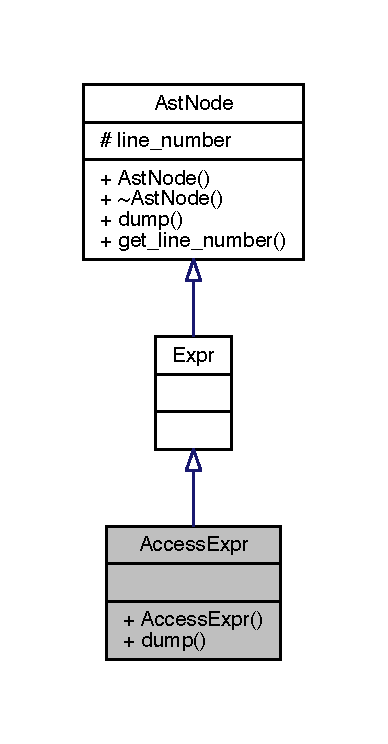
\includegraphics[width=186pt]{class_access_expr__inherit__graph}
\end{center}
\end{figure}


Collaboration diagram for Access\+Expr\+:\nopagebreak
\begin{figure}[H]
\begin{center}
\leavevmode
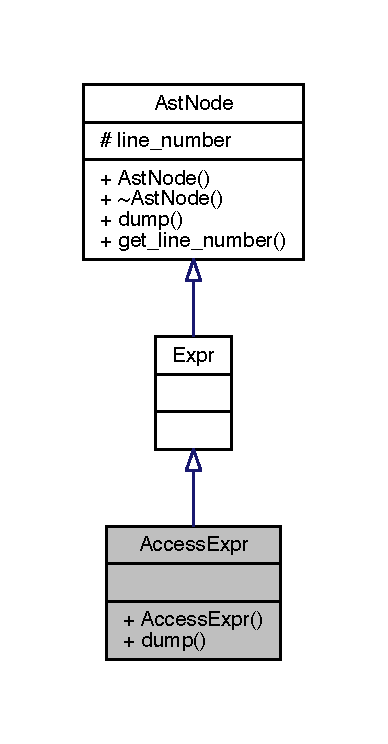
\includegraphics[width=186pt]{class_access_expr__coll__graph}
\end{center}
\end{figure}
\subsection*{Public Member Functions}
\begin{DoxyCompactItemize}
\item 
\mbox{\Hypertarget{class_access_expr_a4b059ca805ab7937cfa02ecf8dd7febb}\label{class_access_expr_a4b059ca805ab7937cfa02ecf8dd7febb}} 
{\bfseries Access\+Expr} (string id, string field)
\item 
\mbox{\Hypertarget{class_access_expr_ae8aeb875cadfe58b833e10eda285019f}\label{class_access_expr_ae8aeb875cadfe58b833e10eda285019f}} 
virtual void {\bfseries dump} (ostream \&os, int n) override
\end{DoxyCompactItemize}
\subsection*{Additional Inherited Members}


The documentation for this class was generated from the following files\+:\begin{DoxyCompactItemize}
\item 
/\+Users/kevin/\+Code/sjtu/smallc/ast.\+h\item 
/\+Users/kevin/\+Code/sjtu/smallc/ast.\+cpp\end{DoxyCompactItemize}

\hypertarget{class_array_init}{}\section{Array\+Init Class Reference}
\label{class_array_init}\index{Array\+Init@{Array\+Init}}


Inheritance diagram for Array\+Init\+:\nopagebreak
\begin{figure}[H]
\begin{center}
\leavevmode
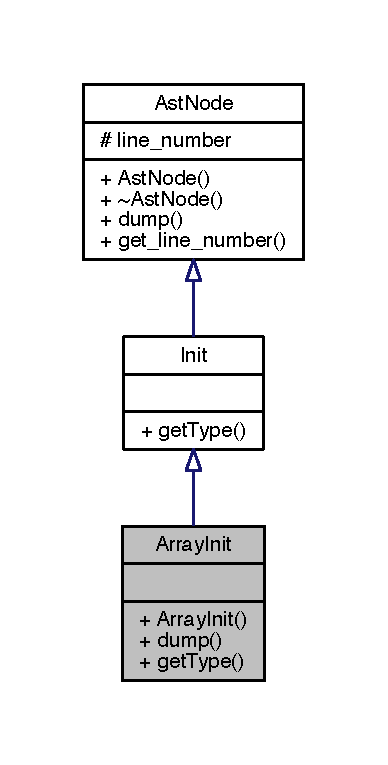
\includegraphics[width=186pt]{class_array_init__inherit__graph}
\end{center}
\end{figure}


Collaboration diagram for Array\+Init\+:\nopagebreak
\begin{figure}[H]
\begin{center}
\leavevmode
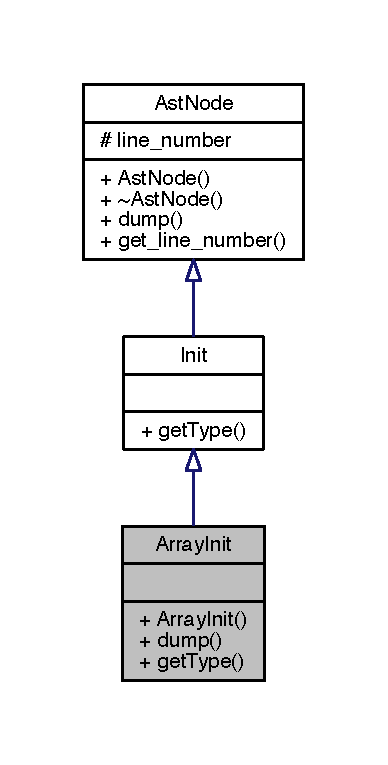
\includegraphics[width=186pt]{class_array_init__coll__graph}
\end{center}
\end{figure}
\subsection*{Public Member Functions}
\begin{DoxyCompactItemize}
\item 
\mbox{\Hypertarget{class_array_init_a89b037692e9f57ebc673591fdd397cf5}\label{class_array_init_a89b037692e9f57ebc673591fdd397cf5}} 
{\bfseries Array\+Init} (Args $\ast$args)
\item 
\mbox{\Hypertarget{class_array_init_acbad83cb15fefc75155c10ed512a209a}\label{class_array_init_acbad83cb15fefc75155c10ed512a209a}} 
virtual void {\bfseries dump} (ostream \&os, int n) override
\item 
\mbox{\Hypertarget{class_array_init_ac7fd7b6aaf5595630deb9ac687867135}\label{class_array_init_ac7fd7b6aaf5595630deb9ac687867135}} 
Expr\+Type\+::type {\bfseries get\+Type} () const override
\end{DoxyCompactItemize}
\subsection*{Additional Inherited Members}


The documentation for this class was generated from the following files\+:\begin{DoxyCompactItemize}
\item 
/\+Users/kevin/\+Code/sjtu/smallc/ast.\+h\item 
/\+Users/kevin/\+Code/sjtu/smallc/ast.\+cpp\end{DoxyCompactItemize}

\hypertarget{class_array_var}{}\section{Array\+Var Class Reference}
\label{class_array_var}\index{Array\+Var@{Array\+Var}}


Inheritance diagram for Array\+Var\+:\nopagebreak
\begin{figure}[H]
\begin{center}
\leavevmode
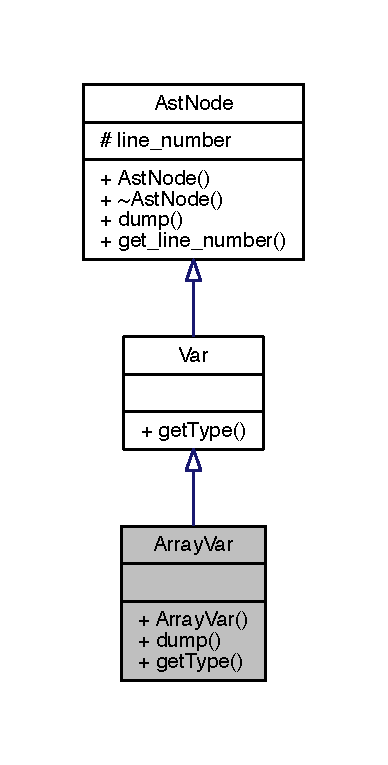
\includegraphics[width=186pt]{class_array_var__inherit__graph}
\end{center}
\end{figure}


Collaboration diagram for Array\+Var\+:\nopagebreak
\begin{figure}[H]
\begin{center}
\leavevmode
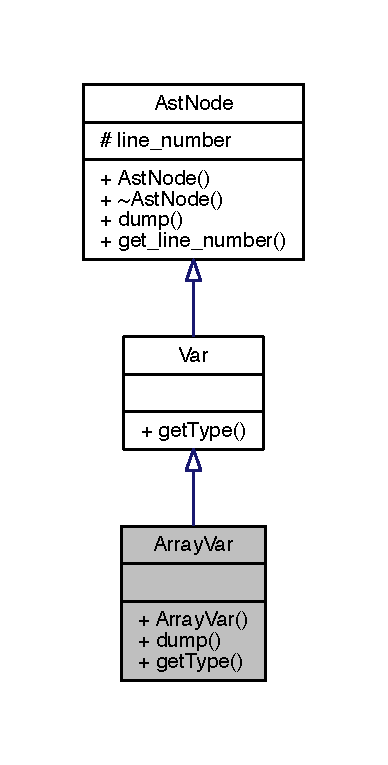
\includegraphics[width=186pt]{class_array_var__coll__graph}
\end{center}
\end{figure}
\subsection*{Public Member Functions}
\begin{DoxyCompactItemize}
\item 
\mbox{\Hypertarget{class_array_var_a1c8b548e48e2e8861352bc09837d9200}\label{class_array_var_a1c8b548e48e2e8861352bc09837d9200}} 
{\bfseries Array\+Var} (\hyperlink{class_var}{Var} $\ast$var, int dim)
\item 
\mbox{\Hypertarget{class_array_var_ac5aa1eec61102a4fdbb1102518b70a1d}\label{class_array_var_ac5aa1eec61102a4fdbb1102518b70a1d}} 
virtual void {\bfseries dump} (ostream \&os, int n) override
\item 
\mbox{\Hypertarget{class_array_var_aa1a9262ecdb395ec8fee2288bde1daf9}\label{class_array_var_aa1a9262ecdb395ec8fee2288bde1daf9}} 
Expr\+Type\+::type {\bfseries get\+Type} () const override
\end{DoxyCompactItemize}
\subsection*{Additional Inherited Members}


The documentation for this class was generated from the following files\+:\begin{DoxyCompactItemize}
\item 
/\+Users/kevin/\+Code/sjtu/smallc/ast.\+h\item 
/\+Users/kevin/\+Code/sjtu/smallc/ast.\+cpp\end{DoxyCompactItemize}

\hypertarget{class_arrs_expr}{}\section{Arrs\+Expr Class Reference}
\label{class_arrs_expr}\index{Arrs\+Expr@{Arrs\+Expr}}


Inheritance diagram for Arrs\+Expr\+:\nopagebreak
\begin{figure}[H]
\begin{center}
\leavevmode
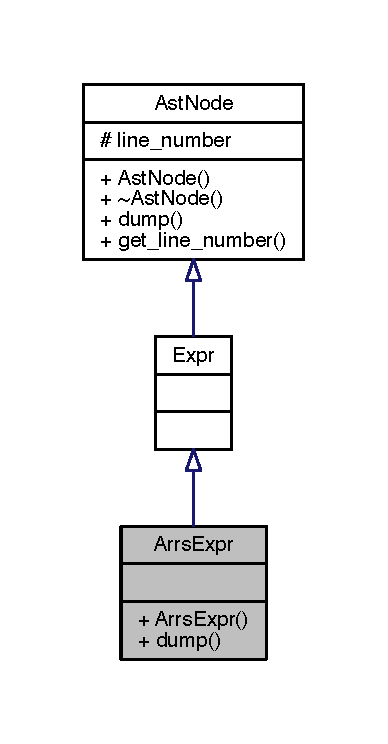
\includegraphics[width=186pt]{class_arrs_expr__inherit__graph}
\end{center}
\end{figure}


Collaboration diagram for Arrs\+Expr\+:\nopagebreak
\begin{figure}[H]
\begin{center}
\leavevmode
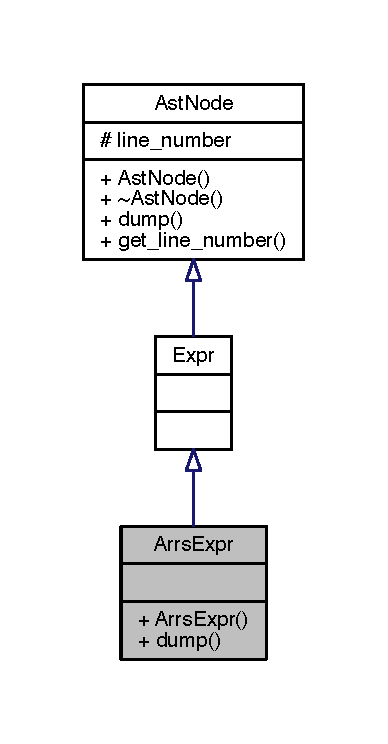
\includegraphics[width=186pt]{class_arrs_expr__coll__graph}
\end{center}
\end{figure}
\subsection*{Public Member Functions}
\begin{DoxyCompactItemize}
\item 
\mbox{\Hypertarget{class_arrs_expr_aad2e2cc9461b024ca57422e3e2ad4009}\label{class_arrs_expr_aad2e2cc9461b024ca57422e3e2ad4009}} 
{\bfseries Arrs\+Expr} (string id, Arrs $\ast$arrs)
\item 
\mbox{\Hypertarget{class_arrs_expr_af1d2325d4a8678c63d94610a20013548}\label{class_arrs_expr_af1d2325d4a8678c63d94610a20013548}} 
virtual void {\bfseries dump} (ostream \&os, int n) override
\end{DoxyCompactItemize}
\subsection*{Additional Inherited Members}


The documentation for this class was generated from the following files\+:\begin{DoxyCompactItemize}
\item 
/\+Users/kevin/\+Code/sjtu/smallc/ast.\+h\item 
/\+Users/kevin/\+Code/sjtu/smallc/ast.\+cpp\end{DoxyCompactItemize}

\hypertarget{class_ast_node}{}\section{Ast\+Node Class Reference}
\label{class_ast_node}\index{Ast\+Node@{Ast\+Node}}


Inheritance diagram for Ast\+Node\+:\nopagebreak
\begin{figure}[H]
\begin{center}
\leavevmode
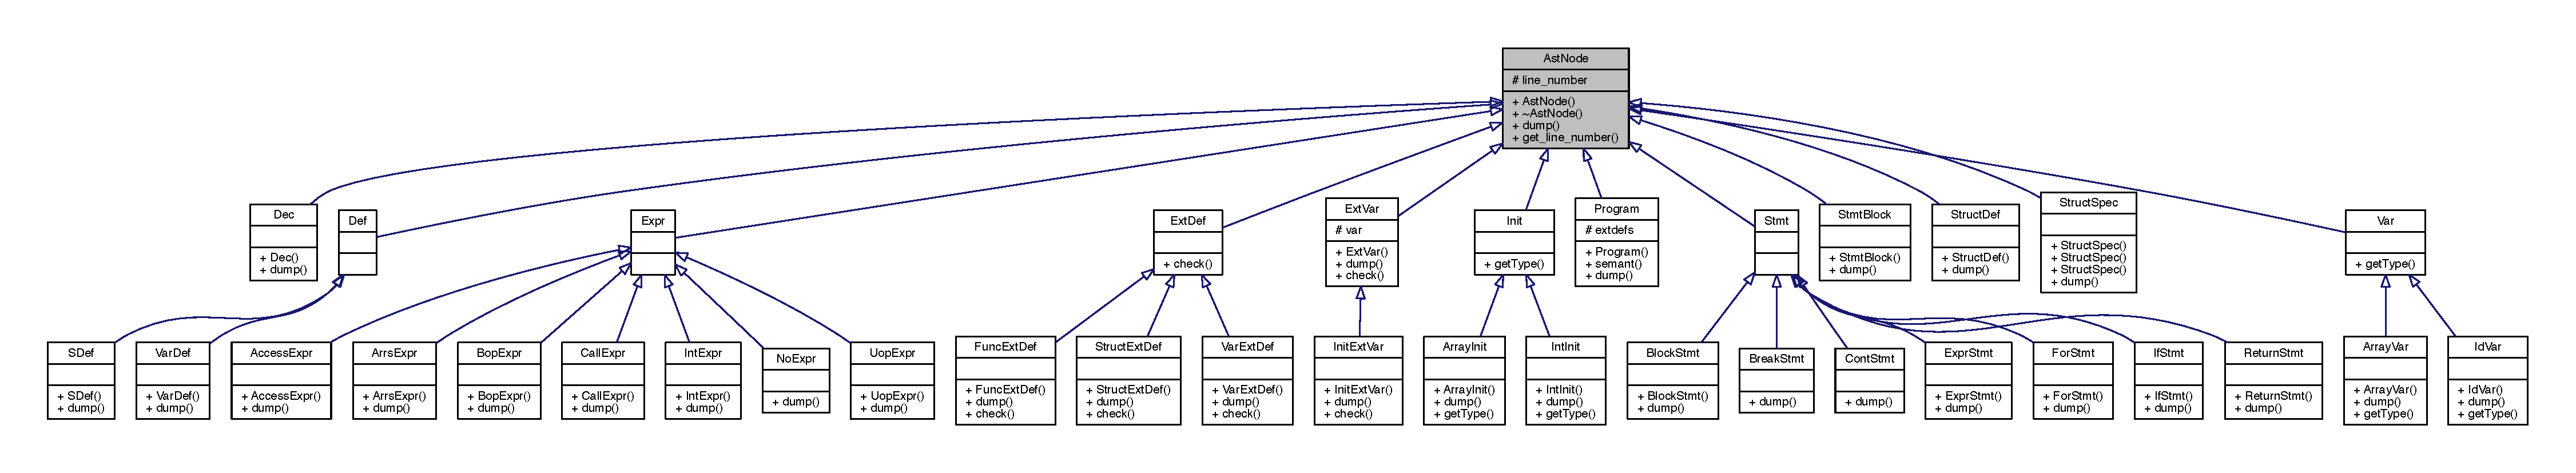
\includegraphics[width=350pt]{class_ast_node__inherit__graph}
\end{center}
\end{figure}


Collaboration diagram for Ast\+Node\+:\nopagebreak
\begin{figure}[H]
\begin{center}
\leavevmode
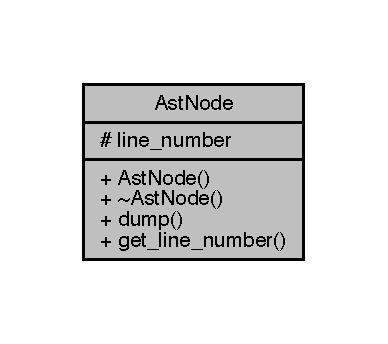
\includegraphics[width=186pt]{class_ast_node__coll__graph}
\end{center}
\end{figure}
\subsection*{Public Member Functions}
\begin{DoxyCompactItemize}
\item 
\mbox{\Hypertarget{class_ast_node_acb1f1b19c076112a17ee276fd2399356}\label{class_ast_node_acb1f1b19c076112a17ee276fd2399356}} 
virtual void {\bfseries dump} (ostream \&os, int n)=0
\item 
\mbox{\Hypertarget{class_ast_node_abc0b47bcba650718684d4277cfae3d9f}\label{class_ast_node_abc0b47bcba650718684d4277cfae3d9f}} 
int {\bfseries get\+\_\+line\+\_\+number} ()
\end{DoxyCompactItemize}
\subsection*{Protected Attributes}
\begin{DoxyCompactItemize}
\item 
\mbox{\Hypertarget{class_ast_node_a2416a4696f3355656a089c7531dec62e}\label{class_ast_node_a2416a4696f3355656a089c7531dec62e}} 
int {\bfseries line\+\_\+number}
\end{DoxyCompactItemize}


The documentation for this class was generated from the following files\+:\begin{DoxyCompactItemize}
\item 
/\+Users/kevin/\+Code/sjtu/smallc/ast.\+h\item 
/\+Users/kevin/\+Code/sjtu/smallc/ast.\+cpp\end{DoxyCompactItemize}

\hypertarget{class_block_stmt}{}\section{Block\+Stmt Class Reference}
\label{class_block_stmt}\index{Block\+Stmt@{Block\+Stmt}}


Inheritance diagram for Block\+Stmt\+:\nopagebreak
\begin{figure}[H]
\begin{center}
\leavevmode
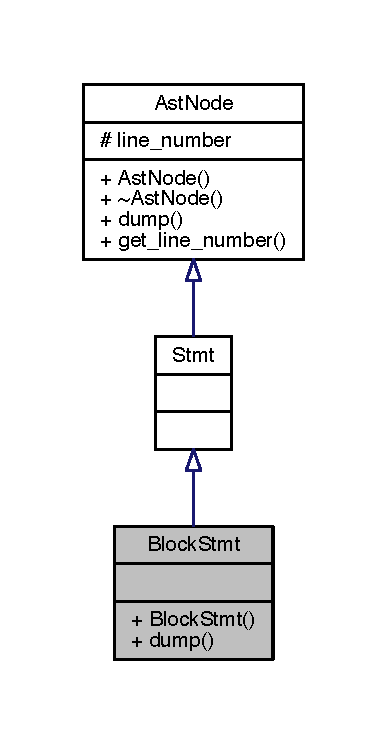
\includegraphics[width=186pt]{class_block_stmt__inherit__graph}
\end{center}
\end{figure}


Collaboration diagram for Block\+Stmt\+:\nopagebreak
\begin{figure}[H]
\begin{center}
\leavevmode
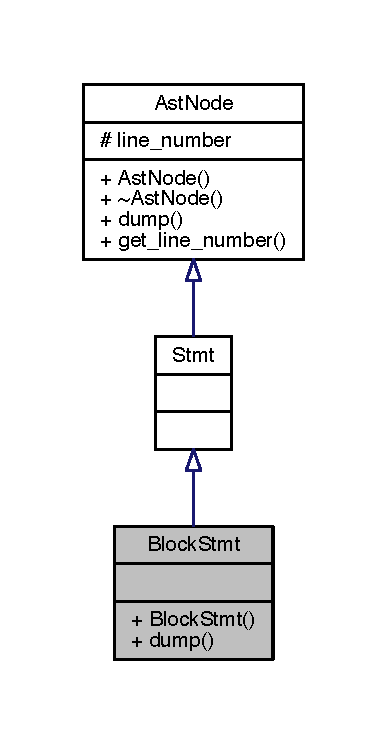
\includegraphics[width=186pt]{class_block_stmt__coll__graph}
\end{center}
\end{figure}
\subsection*{Public Member Functions}
\begin{DoxyCompactItemize}
\item 
\mbox{\Hypertarget{class_block_stmt_a950075376dfde31751d7a6ac17cb4709}\label{class_block_stmt_a950075376dfde31751d7a6ac17cb4709}} 
{\bfseries Block\+Stmt} (\hyperlink{class_stmt_block}{Stmt\+Block} $\ast$sb)
\item 
\mbox{\Hypertarget{class_block_stmt_a698d06bcdd7e81efe08562b62d78672b}\label{class_block_stmt_a698d06bcdd7e81efe08562b62d78672b}} 
virtual void {\bfseries dump} (ostream \&os, int n) override
\end{DoxyCompactItemize}
\subsection*{Additional Inherited Members}


The documentation for this class was generated from the following files\+:\begin{DoxyCompactItemize}
\item 
/\+Users/kevin/\+Code/sjtu/smallc/ast.\+h\item 
/\+Users/kevin/\+Code/sjtu/smallc/ast.\+cpp\end{DoxyCompactItemize}

\hypertarget{class_bop_expr}{}\section{Bop\+Expr Class Reference}
\label{class_bop_expr}\index{Bop\+Expr@{Bop\+Expr}}


Inheritance diagram for Bop\+Expr\+:\nopagebreak
\begin{figure}[H]
\begin{center}
\leavevmode
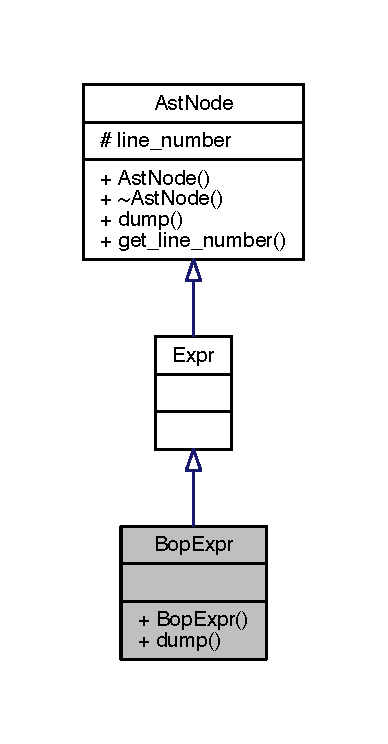
\includegraphics[width=186pt]{class_bop_expr__inherit__graph}
\end{center}
\end{figure}


Collaboration diagram for Bop\+Expr\+:\nopagebreak
\begin{figure}[H]
\begin{center}
\leavevmode
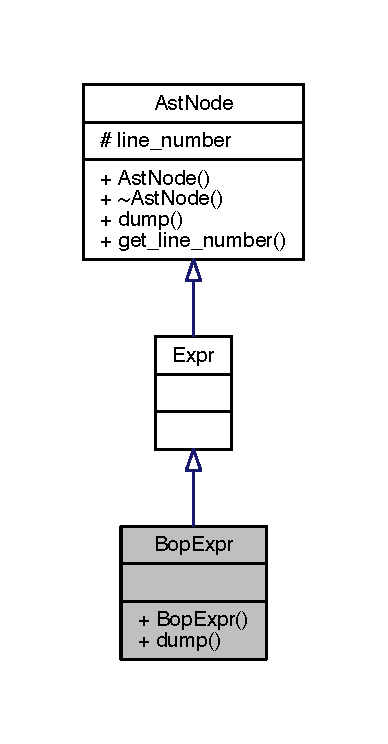
\includegraphics[width=186pt]{class_bop_expr__coll__graph}
\end{center}
\end{figure}
\subsection*{Public Member Functions}
\begin{DoxyCompactItemize}
\item 
\mbox{\Hypertarget{class_bop_expr_a40537ccaae3950e84002a3372fd3bec1}\label{class_bop_expr_a40537ccaae3950e84002a3372fd3bec1}} 
{\bfseries Bop\+Expr} (string op, \hyperlink{class_expr}{Expr} $\ast$lexp, \hyperlink{class_expr}{Expr} $\ast$rexp)
\item 
\mbox{\Hypertarget{class_bop_expr_a26c4b2aabc1e8c43e588b7aea75eee27}\label{class_bop_expr_a26c4b2aabc1e8c43e588b7aea75eee27}} 
virtual void {\bfseries dump} (ostream \&os, int n) override
\end{DoxyCompactItemize}
\subsection*{Additional Inherited Members}


The documentation for this class was generated from the following files\+:\begin{DoxyCompactItemize}
\item 
/\+Users/kevin/\+Code/sjtu/smallc/ast.\+h\item 
/\+Users/kevin/\+Code/sjtu/smallc/ast.\+cpp\end{DoxyCompactItemize}

\hypertarget{class_break_stmt}{}\section{Break\+Stmt Class Reference}
\label{class_break_stmt}\index{Break\+Stmt@{Break\+Stmt}}


Inheritance diagram for Break\+Stmt\+:\nopagebreak
\begin{figure}[H]
\begin{center}
\leavevmode
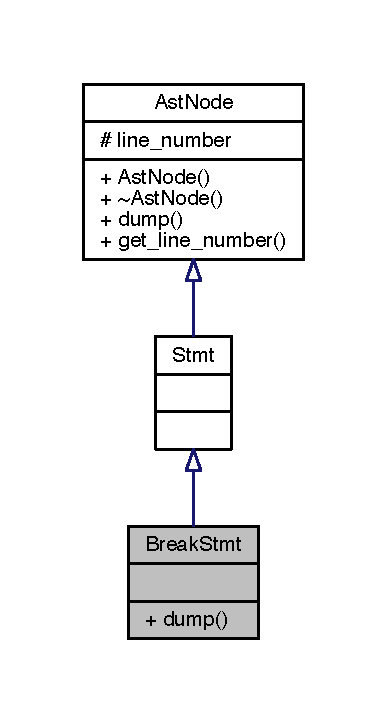
\includegraphics[width=186pt]{class_break_stmt__inherit__graph}
\end{center}
\end{figure}


Collaboration diagram for Break\+Stmt\+:\nopagebreak
\begin{figure}[H]
\begin{center}
\leavevmode
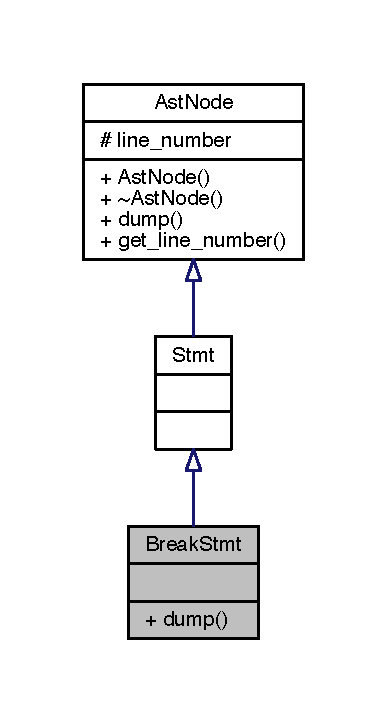
\includegraphics[width=186pt]{class_break_stmt__coll__graph}
\end{center}
\end{figure}
\subsection*{Public Member Functions}
\begin{DoxyCompactItemize}
\item 
\mbox{\Hypertarget{class_break_stmt_aaa03d6bdad0a42890f930e75a4dcb007}\label{class_break_stmt_aaa03d6bdad0a42890f930e75a4dcb007}} 
virtual void {\bfseries dump} (ostream \&os, int n) override
\end{DoxyCompactItemize}
\subsection*{Additional Inherited Members}


The documentation for this class was generated from the following files\+:\begin{DoxyCompactItemize}
\item 
/\+Users/kevin/\+Code/sjtu/smallc/ast.\+h\item 
/\+Users/kevin/\+Code/sjtu/smallc/ast.\+cpp\end{DoxyCompactItemize}

\hypertarget{class_call_expr}{}\section{Call\+Expr Class Reference}
\label{class_call_expr}\index{Call\+Expr@{Call\+Expr}}


Inheritance diagram for Call\+Expr\+:\nopagebreak
\begin{figure}[H]
\begin{center}
\leavevmode
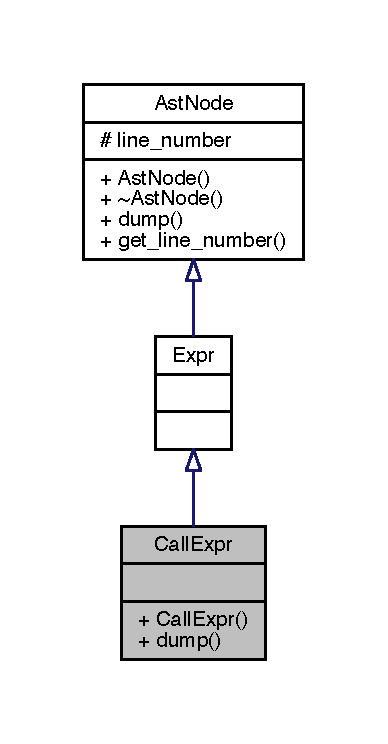
\includegraphics[width=186pt]{class_call_expr__inherit__graph}
\end{center}
\end{figure}


Collaboration diagram for Call\+Expr\+:\nopagebreak
\begin{figure}[H]
\begin{center}
\leavevmode
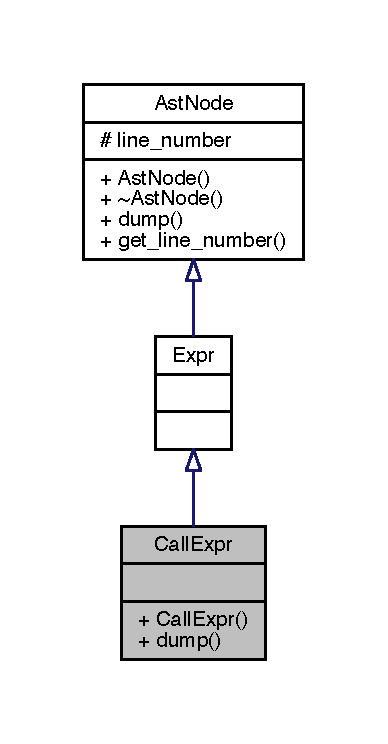
\includegraphics[width=186pt]{class_call_expr__coll__graph}
\end{center}
\end{figure}
\subsection*{Public Member Functions}
\begin{DoxyCompactItemize}
\item 
\mbox{\Hypertarget{class_call_expr_a4717596b2946bec91de14fe27bb66520}\label{class_call_expr_a4717596b2946bec91de14fe27bb66520}} 
{\bfseries Call\+Expr} (string id, Args $\ast$args)
\item 
\mbox{\Hypertarget{class_call_expr_a1dbe2dd41bb5062c2b93b36869aa3083}\label{class_call_expr_a1dbe2dd41bb5062c2b93b36869aa3083}} 
virtual void {\bfseries dump} (ostream \&os, int n) override
\end{DoxyCompactItemize}
\subsection*{Additional Inherited Members}


The documentation for this class was generated from the following files\+:\begin{DoxyCompactItemize}
\item 
/\+Users/kevin/\+Code/sjtu/smallc/ast.\+h\item 
/\+Users/kevin/\+Code/sjtu/smallc/ast.\+cpp\end{DoxyCompactItemize}

\hypertarget{class_cont_stmt}{}\section{Cont\+Stmt Class Reference}
\label{class_cont_stmt}\index{Cont\+Stmt@{Cont\+Stmt}}


Inheritance diagram for Cont\+Stmt\+:\nopagebreak
\begin{figure}[H]
\begin{center}
\leavevmode
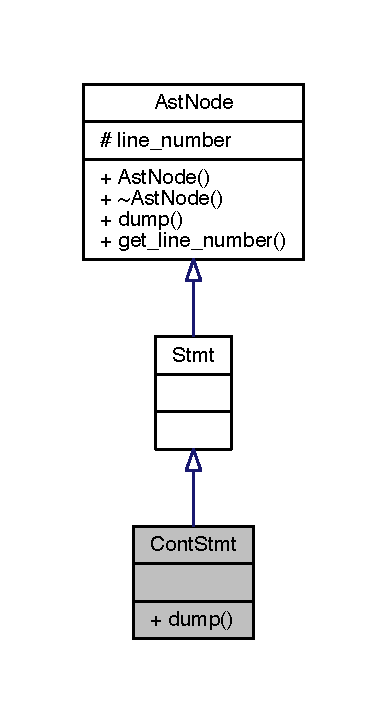
\includegraphics[width=186pt]{class_cont_stmt__inherit__graph}
\end{center}
\end{figure}


Collaboration diagram for Cont\+Stmt\+:\nopagebreak
\begin{figure}[H]
\begin{center}
\leavevmode
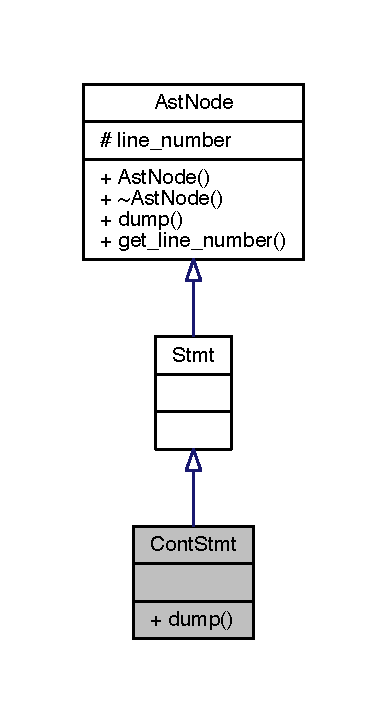
\includegraphics[width=186pt]{class_cont_stmt__coll__graph}
\end{center}
\end{figure}
\subsection*{Public Member Functions}
\begin{DoxyCompactItemize}
\item 
\mbox{\Hypertarget{class_cont_stmt_afb99a6934d38843b50b374b9b47dcb39}\label{class_cont_stmt_afb99a6934d38843b50b374b9b47dcb39}} 
virtual void {\bfseries dump} (ostream \&os, int n) override
\end{DoxyCompactItemize}
\subsection*{Additional Inherited Members}


The documentation for this class was generated from the following files\+:\begin{DoxyCompactItemize}
\item 
/\+Users/kevin/\+Code/sjtu/smallc/ast.\+h\item 
/\+Users/kevin/\+Code/sjtu/smallc/ast.\+cpp\end{DoxyCompactItemize}

\hypertarget{class_dec}{}\section{Dec Class Reference}
\label{class_dec}\index{Dec@{Dec}}


{\ttfamily \#include $<$ast.\+h$>$}



Inheritance diagram for Dec\+:\nopagebreak
\begin{figure}[H]
\begin{center}
\leavevmode
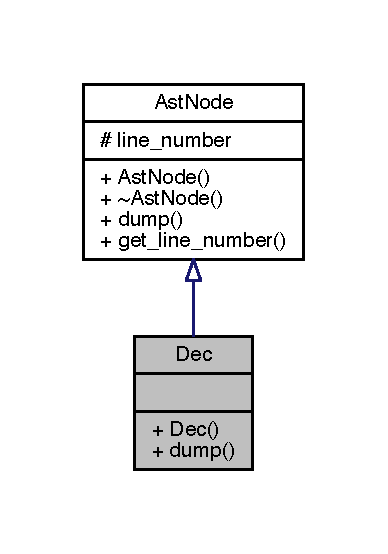
\includegraphics[width=186pt]{class_dec__inherit__graph}
\end{center}
\end{figure}


Collaboration diagram for Dec\+:\nopagebreak
\begin{figure}[H]
\begin{center}
\leavevmode
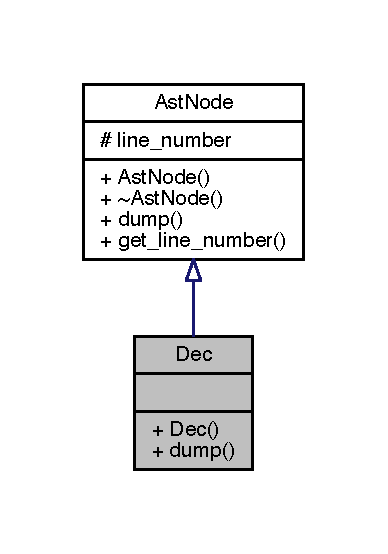
\includegraphics[width=186pt]{class_dec__coll__graph}
\end{center}
\end{figure}
\subsection*{Public Member Functions}
\begin{DoxyCompactItemize}
\item 
\mbox{\Hypertarget{class_dec_a272e415617fe422cd8301bd5fcefd2ef}\label{class_dec_a272e415617fe422cd8301bd5fcefd2ef}} 
{\bfseries Dec} (\hyperlink{class_var}{Var} $\ast$v, \hyperlink{class_init}{Init} $\ast$in=nullptr)
\item 
\mbox{\Hypertarget{class_dec_aa776c5bb5bc8596a798ef491105996f0}\label{class_dec_aa776c5bb5bc8596a798ef491105996f0}} 
virtual void {\bfseries dump} (ostream \&os, int n) override
\end{DoxyCompactItemize}
\subsection*{Additional Inherited Members}


\subsection{Detailed Description}
D\+EC -\/$>$ V\+AR $\vert$ V\+AR A\+S\+S\+I\+GN I\+N\+IT 

The documentation for this class was generated from the following files\+:\begin{DoxyCompactItemize}
\item 
/\+Users/kevin/\+Code/sjtu/smallc/ast.\+h\item 
/\+Users/kevin/\+Code/sjtu/smallc/ast.\+cpp\end{DoxyCompactItemize}

\hypertarget{class_def}{}\section{Def Class Reference}
\label{class_def}\index{Def@{Def}}


{\ttfamily \#include $<$ast.\+h$>$}



Inheritance diagram for Def\+:\nopagebreak
\begin{figure}[H]
\begin{center}
\leavevmode
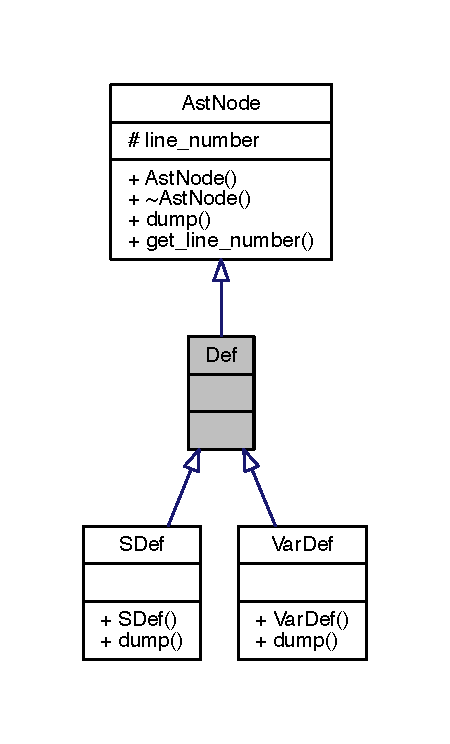
\includegraphics[width=216pt]{class_def__inherit__graph}
\end{center}
\end{figure}


Collaboration diagram for Def\+:\nopagebreak
\begin{figure}[H]
\begin{center}
\leavevmode
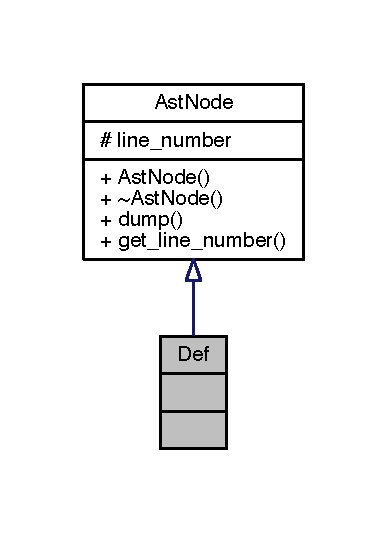
\includegraphics[width=186pt]{class_def__coll__graph}
\end{center}
\end{figure}
\subsection*{Additional Inherited Members}


\subsection{Detailed Description}
\hyperlink{class_def}{Def}

D\+EF -\/$>$ T\+Y\+PE D\+E\+CS S\+E\+MI $\sim$ \hyperlink{class_var_def}{Var\+Def} $\vert$ S\+T\+S\+P\+EC S\+D\+E\+CS S\+E\+MI $\sim$ \hyperlink{class_s_def}{S\+Def} 

The documentation for this class was generated from the following file\+:\begin{DoxyCompactItemize}
\item 
/\+Users/kevin/\+Code/sjtu/smallc/ast.\+h\end{DoxyCompactItemize}

\hypertarget{class_expr}{}\section{Expr Class Reference}
\label{class_expr}\index{Expr@{Expr}}


{\ttfamily \#include $<$ast.\+h$>$}



Inheritance diagram for Expr\+:\nopagebreak
\begin{figure}[H]
\begin{center}
\leavevmode
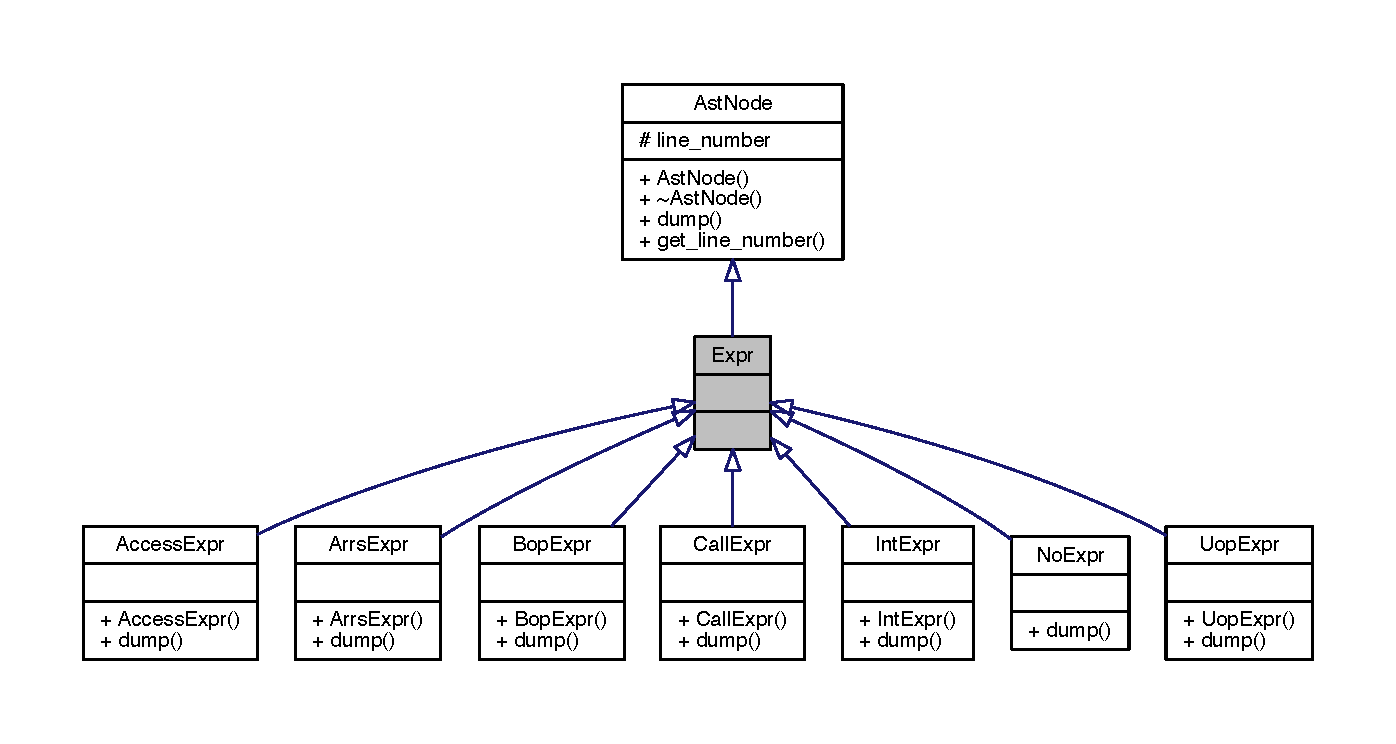
\includegraphics[width=350pt]{class_expr__inherit__graph}
\end{center}
\end{figure}


Collaboration diagram for Expr\+:\nopagebreak
\begin{figure}[H]
\begin{center}
\leavevmode
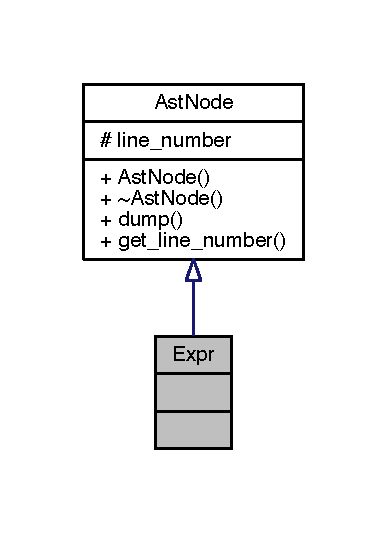
\includegraphics[width=186pt]{class_expr__coll__graph}
\end{center}
\end{figure}
\subsection*{Additional Inherited Members}


\subsection{Detailed Description}
\hyperlink{class_expr}{Expr} 

The documentation for this class was generated from the following file\+:\begin{DoxyCompactItemize}
\item 
/\+Users/kevin/\+Code/sjtu/smallc/ast.\+h\end{DoxyCompactItemize}

\hypertarget{class_expr_stmt}{}\section{Expr\+Stmt Class Reference}
\label{class_expr_stmt}\index{Expr\+Stmt@{Expr\+Stmt}}


Inheritance diagram for Expr\+Stmt\+:\nopagebreak
\begin{figure}[H]
\begin{center}
\leavevmode
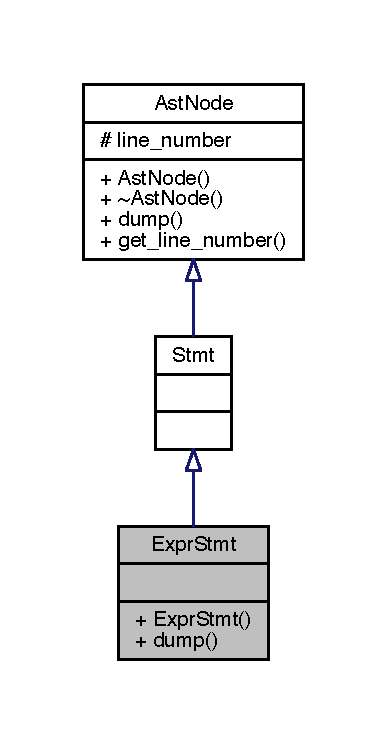
\includegraphics[width=186pt]{class_expr_stmt__inherit__graph}
\end{center}
\end{figure}


Collaboration diagram for Expr\+Stmt\+:\nopagebreak
\begin{figure}[H]
\begin{center}
\leavevmode
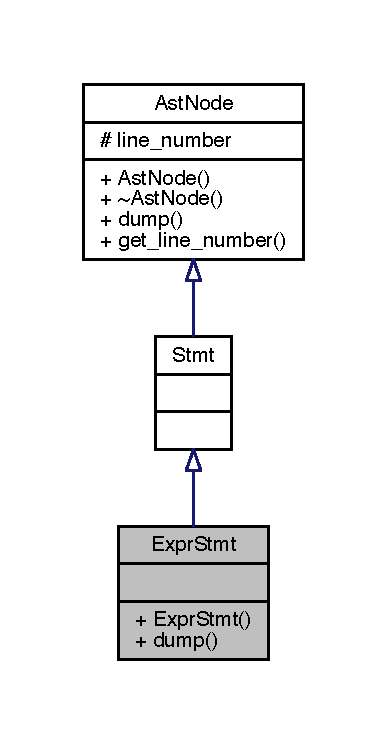
\includegraphics[width=186pt]{class_expr_stmt__coll__graph}
\end{center}
\end{figure}
\subsection*{Public Member Functions}
\begin{DoxyCompactItemize}
\item 
\mbox{\Hypertarget{class_expr_stmt_aed258a5f037345f06b6a9962c8a43514}\label{class_expr_stmt_aed258a5f037345f06b6a9962c8a43514}} 
{\bfseries Expr\+Stmt} (\hyperlink{class_expr}{Expr} $\ast$exp)
\item 
\mbox{\Hypertarget{class_expr_stmt_a9bf6da4398579a653e547d2ace3493d0}\label{class_expr_stmt_a9bf6da4398579a653e547d2ace3493d0}} 
virtual void {\bfseries dump} (ostream \&os, int n) override
\end{DoxyCompactItemize}
\subsection*{Additional Inherited Members}


The documentation for this class was generated from the following files\+:\begin{DoxyCompactItemize}
\item 
/\+Users/kevin/\+Code/sjtu/smallc/ast.\+h\item 
/\+Users/kevin/\+Code/sjtu/smallc/ast.\+cpp\end{DoxyCompactItemize}

\hypertarget{class_ext_def}{}\section{Ext\+Def Class Reference}
\label{class_ext_def}\index{Ext\+Def@{Ext\+Def}}


{\ttfamily \#include $<$ast.\+h$>$}



Inheritance diagram for Ext\+Def\+:\nopagebreak
\begin{figure}[H]
\begin{center}
\leavevmode
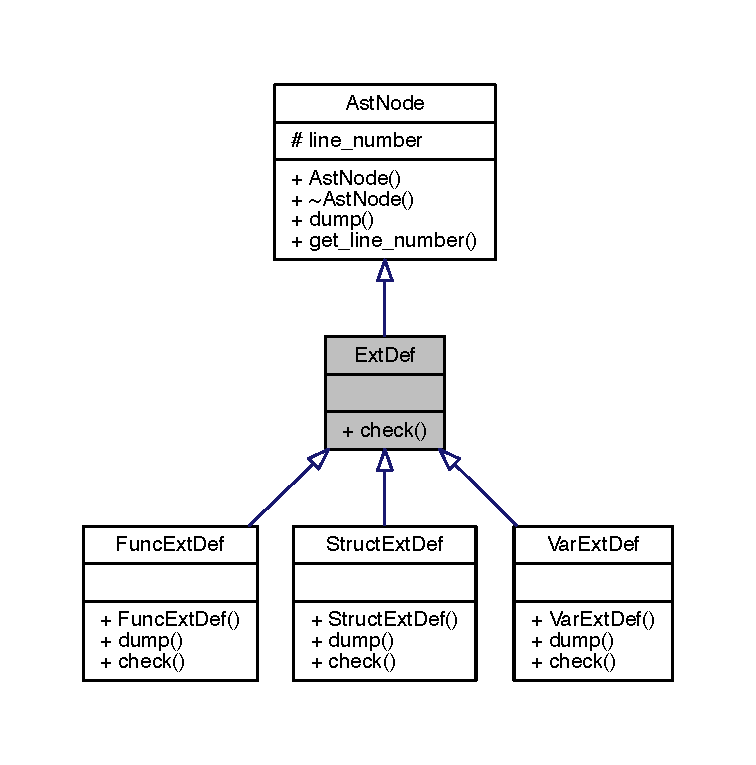
\includegraphics[width=350pt]{class_ext_def__inherit__graph}
\end{center}
\end{figure}


Collaboration diagram for Ext\+Def\+:\nopagebreak
\begin{figure}[H]
\begin{center}
\leavevmode
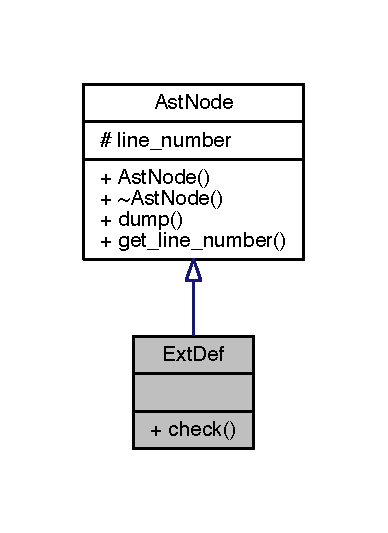
\includegraphics[width=186pt]{class_ext_def__coll__graph}
\end{center}
\end{figure}
\subsection*{Public Member Functions}
\begin{DoxyCompactItemize}
\item 
\mbox{\Hypertarget{class_ext_def_a1b764d99bfc974bd261d7f0b6e141132}\label{class_ext_def_a1b764d99bfc974bd261d7f0b6e141132}} 
virtual void {\bfseries check} ()=0
\end{DoxyCompactItemize}
\subsection*{Additional Inherited Members}


\subsection{Detailed Description}
E\+X\+T\+D\+EF -\/$>$ T\+Y\+PE E\+X\+T\+V\+A\+RS S\+E\+MI $\sim$ \hyperlink{class_var_ext_def}{Var\+Ext\+Def} $\vert$ S\+T\+S\+P\+EC S\+E\+X\+T\+V\+A\+RS S\+E\+MI $\sim$ \hyperlink{class_struct_ext_def}{Struct\+Ext\+Def} $\vert$ T\+Y\+PE ID LP P\+A\+R\+AS RP S\+T\+M\+T\+B\+L\+O\+CK $\sim$ \hyperlink{class_func_ext_def}{Func\+Ext\+Def} 

The documentation for this class was generated from the following file\+:\begin{DoxyCompactItemize}
\item 
/\+Users/kevin/\+Code/sjtu/smallc/ast.\+h\end{DoxyCompactItemize}

\hypertarget{class_ext_var}{}\section{Ext\+Var Class Reference}
\label{class_ext_var}\index{Ext\+Var@{Ext\+Var}}


{\ttfamily \#include $<$ast.\+h$>$}



Inheritance diagram for Ext\+Var\+:\nopagebreak
\begin{figure}[H]
\begin{center}
\leavevmode
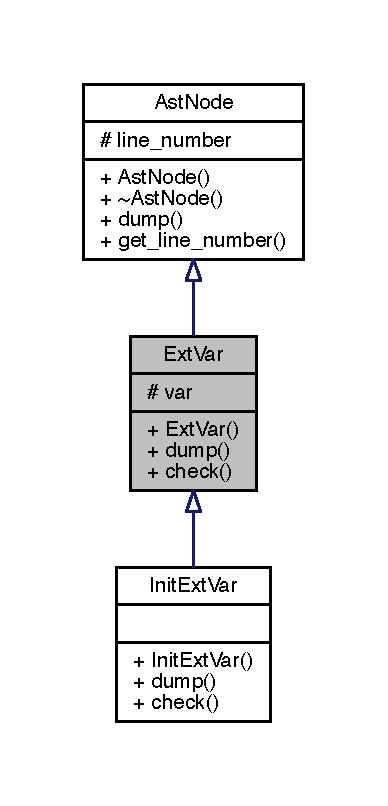
\includegraphics[width=186pt]{class_ext_var__inherit__graph}
\end{center}
\end{figure}


Collaboration diagram for Ext\+Var\+:\nopagebreak
\begin{figure}[H]
\begin{center}
\leavevmode
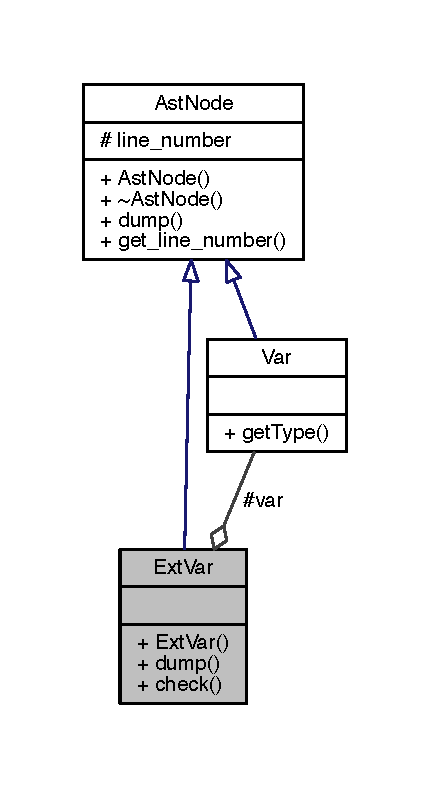
\includegraphics[width=206pt]{class_ext_var__coll__graph}
\end{center}
\end{figure}
\subsection*{Public Member Functions}
\begin{DoxyCompactItemize}
\item 
\mbox{\Hypertarget{class_ext_var_abb6174d2fdfb84b434f95172dfd0076c}\label{class_ext_var_abb6174d2fdfb84b434f95172dfd0076c}} 
{\bfseries Ext\+Var} (\hyperlink{class_var}{Var} $\ast$var)
\item 
\mbox{\Hypertarget{class_ext_var_af75fe07af96da67a210f4601589d5d1b}\label{class_ext_var_af75fe07af96da67a210f4601589d5d1b}} 
virtual void {\bfseries dump} (ostream \&os, int n) override
\item 
\mbox{\Hypertarget{class_ext_var_a98ba57934575d616f570021e644ae071}\label{class_ext_var_a98ba57934575d616f570021e644ae071}} 
virtual void {\bfseries check} ()
\end{DoxyCompactItemize}
\subsection*{Protected Attributes}
\begin{DoxyCompactItemize}
\item 
\mbox{\Hypertarget{class_ext_var_af3338fd1abf1a794cd1f24e7eed81b78}\label{class_ext_var_af3338fd1abf1a794cd1f24e7eed81b78}} 
\hyperlink{class_var}{Var} $\ast$ {\bfseries var}
\end{DoxyCompactItemize}


\subsection{Detailed Description}
\hyperlink{class_ext_var}{Ext\+Var}

E\+X\+T\+V\+AR -\/$>$ V\+AR $\sim$ \hyperlink{class_ext_var}{Ext\+Var} $\vert$ V\+AR A\+S\+S\+I\+GN I\+N\+IT $\sim$ \hyperlink{class_init_ext_var}{Init\+Ext\+Var} 

The documentation for this class was generated from the following files\+:\begin{DoxyCompactItemize}
\item 
/\+Users/kevin/\+Code/sjtu/smallc/ast.\+h\item 
/\+Users/kevin/\+Code/sjtu/smallc/ast.\+cpp\end{DoxyCompactItemize}

\hypertarget{class_for_stmt}{}\section{For\+Stmt Class Reference}
\label{class_for_stmt}\index{For\+Stmt@{For\+Stmt}}


Inheritance diagram for For\+Stmt\+:\nopagebreak
\begin{figure}[H]
\begin{center}
\leavevmode
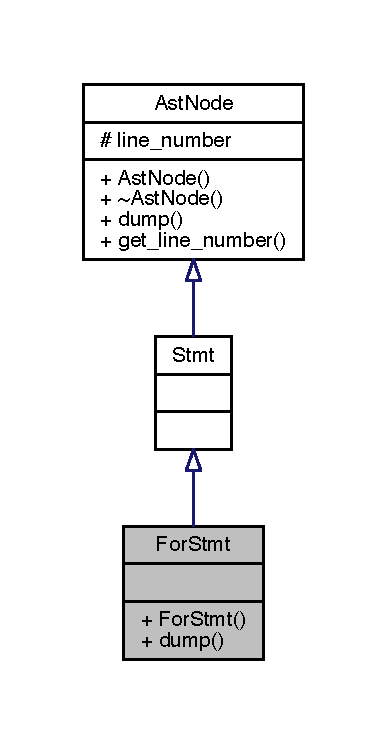
\includegraphics[width=186pt]{class_for_stmt__inherit__graph}
\end{center}
\end{figure}


Collaboration diagram for For\+Stmt\+:\nopagebreak
\begin{figure}[H]
\begin{center}
\leavevmode
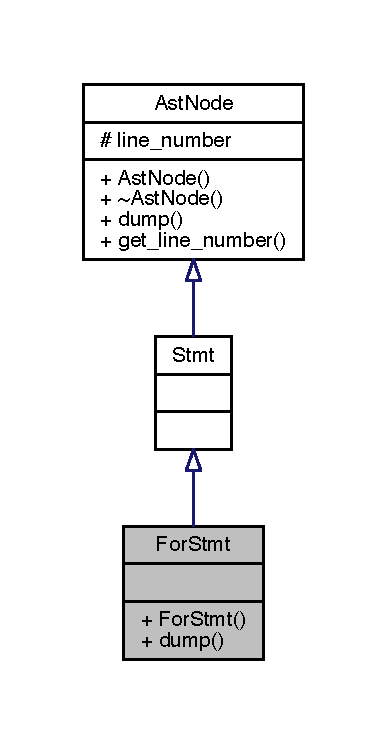
\includegraphics[width=186pt]{class_for_stmt__coll__graph}
\end{center}
\end{figure}
\subsection*{Public Member Functions}
\begin{DoxyCompactItemize}
\item 
\mbox{\Hypertarget{class_for_stmt_a4344848679ad4a9a24c2af926cd2fbaa}\label{class_for_stmt_a4344848679ad4a9a24c2af926cd2fbaa}} 
{\bfseries For\+Stmt} (\hyperlink{class_expr}{Expr} $\ast$e1, \hyperlink{class_expr}{Expr} $\ast$e2, \hyperlink{class_expr}{Expr} $\ast$e3, \hyperlink{class_stmt}{Stmt} $\ast$stmt)
\item 
\mbox{\Hypertarget{class_for_stmt_ad271254d3347f7eff979e207bd815ce0}\label{class_for_stmt_ad271254d3347f7eff979e207bd815ce0}} 
virtual void {\bfseries dump} (ostream \&os, int n) override
\end{DoxyCompactItemize}
\subsection*{Additional Inherited Members}


The documentation for this class was generated from the following files\+:\begin{DoxyCompactItemize}
\item 
/\+Users/kevin/\+Code/sjtu/smallc/ast.\+h\item 
/\+Users/kevin/\+Code/sjtu/smallc/ast.\+cpp\end{DoxyCompactItemize}

\hypertarget{class_func_ext_def}{}\section{Func\+Ext\+Def Class Reference}
\label{class_func_ext_def}\index{Func\+Ext\+Def@{Func\+Ext\+Def}}


{\ttfamily \#include $<$ast.\+h$>$}



Inheritance diagram for Func\+Ext\+Def\+:\nopagebreak
\begin{figure}[H]
\begin{center}
\leavevmode
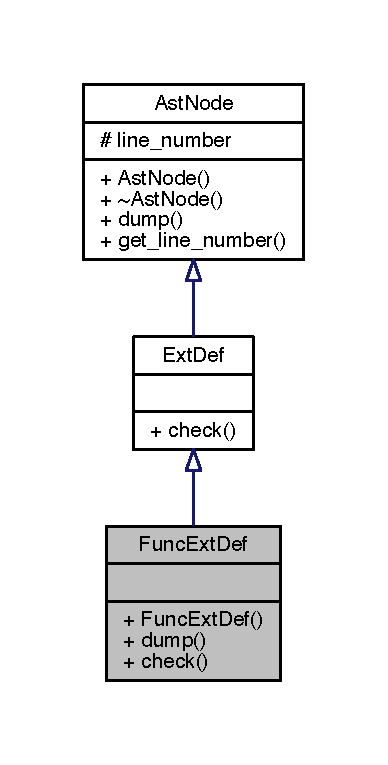
\includegraphics[width=186pt]{class_func_ext_def__inherit__graph}
\end{center}
\end{figure}


Collaboration diagram for Func\+Ext\+Def\+:\nopagebreak
\begin{figure}[H]
\begin{center}
\leavevmode
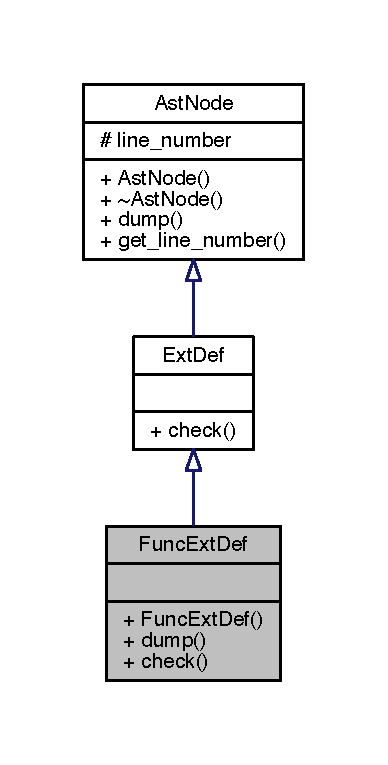
\includegraphics[width=186pt]{class_func_ext_def__coll__graph}
\end{center}
\end{figure}
\subsection*{Public Member Functions}
\begin{DoxyCompactItemize}
\item 
\mbox{\Hypertarget{class_func_ext_def_aa937c117fe72eae933276738f7406ceb}\label{class_func_ext_def_aa937c117fe72eae933276738f7406ceb}} 
{\bfseries Func\+Ext\+Def} (string id, Paras $\ast$p, \hyperlink{class_stmt_block}{Stmt\+Block} $\ast$stmt\+Block)
\item 
\mbox{\Hypertarget{class_func_ext_def_a24f3b7f5d389ac97bea09c5b7332ce03}\label{class_func_ext_def_a24f3b7f5d389ac97bea09c5b7332ce03}} 
virtual void {\bfseries dump} (ostream \&os, int n) override
\item 
\mbox{\Hypertarget{class_func_ext_def_ac768526c6373721de90662322ccc1470}\label{class_func_ext_def_ac768526c6373721de90662322ccc1470}} 
void {\bfseries check} () override
\end{DoxyCompactItemize}
\subsection*{Additional Inherited Members}


\subsection{Detailed Description}
Function defs

E\+X\+T\+D\+EF -\/$>$ T\+Y\+PE ID LP P\+A\+R\+AS RP S\+T\+M\+T\+B\+L\+O\+CK 

The documentation for this class was generated from the following files\+:\begin{DoxyCompactItemize}
\item 
/\+Users/kevin/\+Code/sjtu/smallc/ast.\+h\item 
/\+Users/kevin/\+Code/sjtu/smallc/ast.\+cpp\end{DoxyCompactItemize}

\hypertarget{class_id_var}{}\section{Id\+Var Class Reference}
\label{class_id_var}\index{Id\+Var@{Id\+Var}}


Inheritance diagram for Id\+Var\+:\nopagebreak
\begin{figure}[H]
\begin{center}
\leavevmode
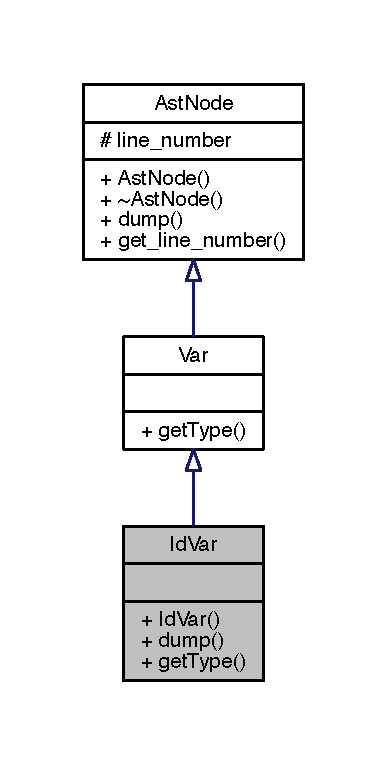
\includegraphics[width=186pt]{class_id_var__inherit__graph}
\end{center}
\end{figure}


Collaboration diagram for Id\+Var\+:\nopagebreak
\begin{figure}[H]
\begin{center}
\leavevmode
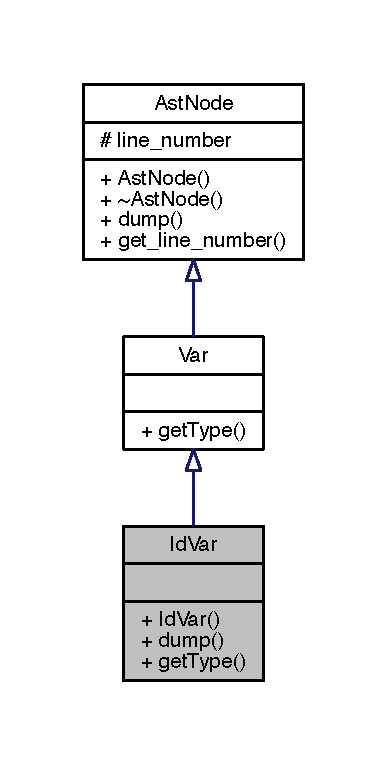
\includegraphics[width=186pt]{class_id_var__coll__graph}
\end{center}
\end{figure}
\subsection*{Public Member Functions}
\begin{DoxyCompactItemize}
\item 
\mbox{\Hypertarget{class_id_var_a6fcaa618b1bd04acb3cae1f42bd8536a}\label{class_id_var_a6fcaa618b1bd04acb3cae1f42bd8536a}} 
{\bfseries Id\+Var} (string id)
\item 
\mbox{\Hypertarget{class_id_var_a60a26d450fd1d269f0462444a90054cf}\label{class_id_var_a60a26d450fd1d269f0462444a90054cf}} 
virtual void {\bfseries dump} (ostream \&os, int n) override
\item 
\mbox{\Hypertarget{class_id_var_a1a965ceb0bd0f3856ef7f1dde75b5c6e}\label{class_id_var_a1a965ceb0bd0f3856ef7f1dde75b5c6e}} 
Expr\+Type\+::type {\bfseries get\+Type} () const override
\end{DoxyCompactItemize}
\subsection*{Additional Inherited Members}


The documentation for this class was generated from the following files\+:\begin{DoxyCompactItemize}
\item 
/\+Users/kevin/\+Code/sjtu/smallc/ast.\+h\item 
/\+Users/kevin/\+Code/sjtu/smallc/ast.\+cpp\end{DoxyCompactItemize}

\hypertarget{class_if_stmt}{}\section{If\+Stmt Class Reference}
\label{class_if_stmt}\index{If\+Stmt@{If\+Stmt}}


Inheritance diagram for If\+Stmt\+:\nopagebreak
\begin{figure}[H]
\begin{center}
\leavevmode
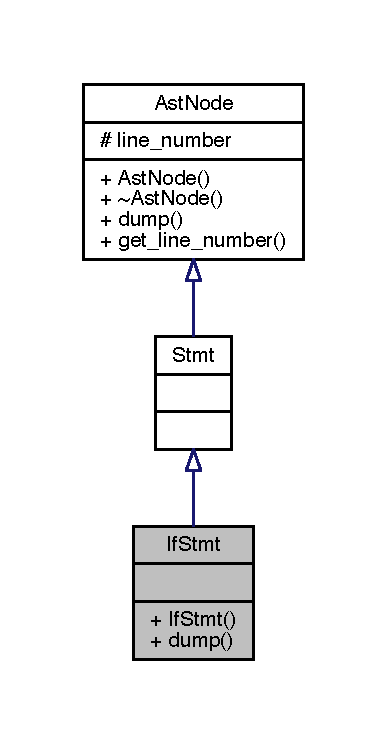
\includegraphics[width=186pt]{class_if_stmt__inherit__graph}
\end{center}
\end{figure}


Collaboration diagram for If\+Stmt\+:\nopagebreak
\begin{figure}[H]
\begin{center}
\leavevmode
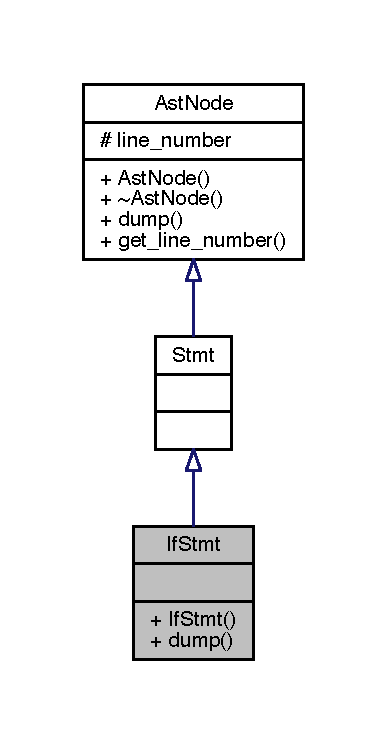
\includegraphics[width=186pt]{class_if_stmt__coll__graph}
\end{center}
\end{figure}
\subsection*{Public Member Functions}
\begin{DoxyCompactItemize}
\item 
\mbox{\Hypertarget{class_if_stmt_a67184c90f8121a9d37e2425869cad659}\label{class_if_stmt_a67184c90f8121a9d37e2425869cad659}} 
{\bfseries If\+Stmt} (\hyperlink{class_expr}{Expr} $\ast$cond, \hyperlink{class_stmt}{Stmt} $\ast$ts, \hyperlink{class_stmt}{Stmt} $\ast$es=nullptr)
\item 
\mbox{\Hypertarget{class_if_stmt_a439420ca9fd3c58fa6830292bb63c886}\label{class_if_stmt_a439420ca9fd3c58fa6830292bb63c886}} 
virtual void {\bfseries dump} (ostream \&os, int n) override
\end{DoxyCompactItemize}
\subsection*{Additional Inherited Members}


The documentation for this class was generated from the following files\+:\begin{DoxyCompactItemize}
\item 
/\+Users/kevin/\+Code/sjtu/smallc/ast.\+h\item 
/\+Users/kevin/\+Code/sjtu/smallc/ast.\+cpp\end{DoxyCompactItemize}

\hypertarget{class_init}{}\section{Init Class Reference}
\label{class_init}\index{Init@{Init}}


{\ttfamily \#include $<$ast.\+h$>$}



Inheritance diagram for Init\+:\nopagebreak
\begin{figure}[H]
\begin{center}
\leavevmode
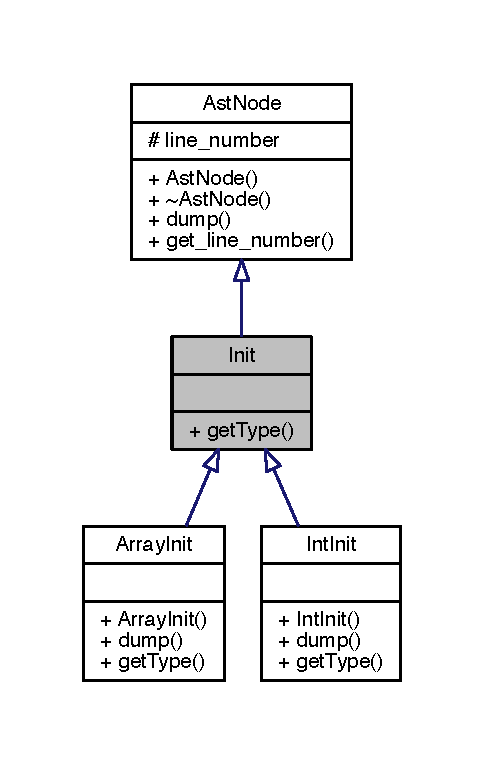
\includegraphics[width=232pt]{class_init__inherit__graph}
\end{center}
\end{figure}


Collaboration diagram for Init\+:\nopagebreak
\begin{figure}[H]
\begin{center}
\leavevmode
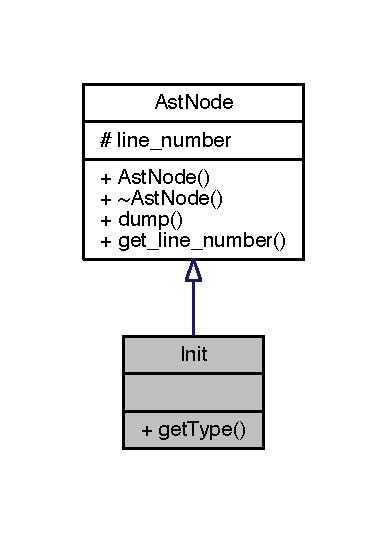
\includegraphics[width=186pt]{class_init__coll__graph}
\end{center}
\end{figure}
\subsection*{Public Member Functions}
\begin{DoxyCompactItemize}
\item 
\mbox{\Hypertarget{class_init_a6eafedc3e8a1797cb1ac780438acdd31}\label{class_init_a6eafedc3e8a1797cb1ac780438acdd31}} 
virtual Expr\+Type\+::type {\bfseries get\+Type} () const
\end{DoxyCompactItemize}
\subsection*{Additional Inherited Members}


\subsection{Detailed Description}
\hyperlink{class_init}{Init}

I\+N\+IT -\/$>$ E\+XP $\sim$ \hyperlink{class_int_init}{Int\+Init} $\vert$ LC A\+R\+GS RC $\sim$ \hyperlink{class_array_init}{Array\+Init} 

The documentation for this class was generated from the following file\+:\begin{DoxyCompactItemize}
\item 
/\+Users/kevin/\+Code/sjtu/smallc/ast.\+h\end{DoxyCompactItemize}

\hypertarget{class_init_ext_var}{}\section{Init\+Ext\+Var Class Reference}
\label{class_init_ext_var}\index{Init\+Ext\+Var@{Init\+Ext\+Var}}


{\ttfamily \#include $<$ast.\+h$>$}



Inheritance diagram for Init\+Ext\+Var\+:\nopagebreak
\begin{figure}[H]
\begin{center}
\leavevmode
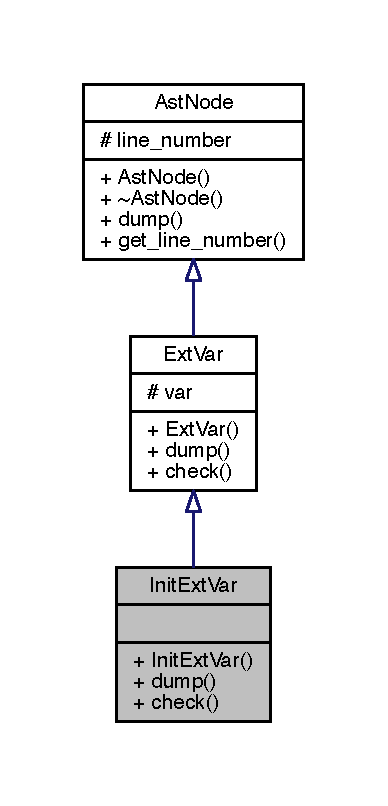
\includegraphics[width=186pt]{class_init_ext_var__inherit__graph}
\end{center}
\end{figure}


Collaboration diagram for Init\+Ext\+Var\+:\nopagebreak
\begin{figure}[H]
\begin{center}
\leavevmode
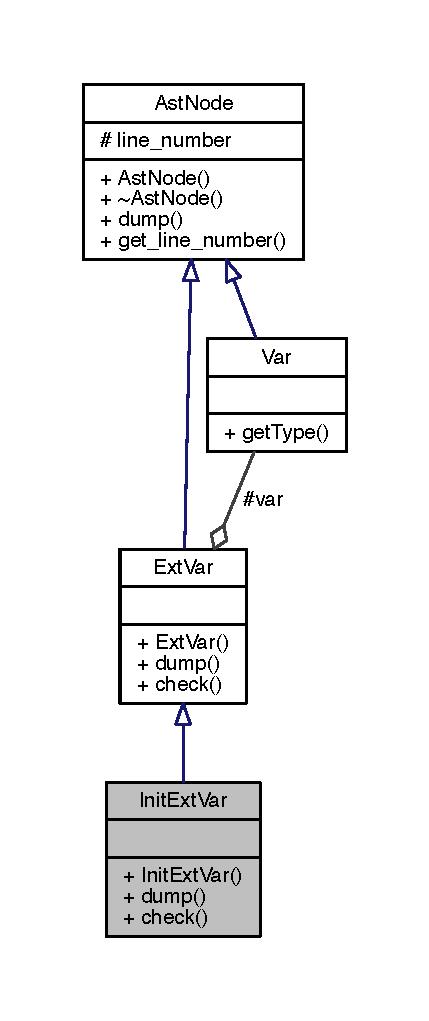
\includegraphics[width=206pt]{class_init_ext_var__coll__graph}
\end{center}
\end{figure}
\subsection*{Public Member Functions}
\begin{DoxyCompactItemize}
\item 
\mbox{\Hypertarget{class_init_ext_var_ad09db3bbb7b681f7c78d5802fa0b2e04}\label{class_init_ext_var_ad09db3bbb7b681f7c78d5802fa0b2e04}} 
{\bfseries Init\+Ext\+Var} (\hyperlink{class_var}{Var} $\ast$pvar, \hyperlink{class_init}{Init} $\ast$pinit)
\item 
\mbox{\Hypertarget{class_init_ext_var_ad4c4e8b8efb98754aead61e70443d518}\label{class_init_ext_var_ad4c4e8b8efb98754aead61e70443d518}} 
virtual void {\bfseries dump} (ostream \&os, int n) override
\item 
\mbox{\Hypertarget{class_init_ext_var_a98f9e53776db14c29260d59a73c8a3be}\label{class_init_ext_var_a98f9e53776db14c29260d59a73c8a3be}} 
void {\bfseries check} () override
\end{DoxyCompactItemize}
\subsection*{Additional Inherited Members}


\subsection{Detailed Description}
E\+X\+T\+V\+AR -\/$>$ V\+AR A\+S\+S\+I\+GN I\+N\+IT 

The documentation for this class was generated from the following files\+:\begin{DoxyCompactItemize}
\item 
/\+Users/kevin/\+Code/sjtu/smallc/ast.\+h\item 
/\+Users/kevin/\+Code/sjtu/smallc/ast.\+cpp\end{DoxyCompactItemize}

\hypertarget{class_int_expr}{}\section{Int\+Expr Class Reference}
\label{class_int_expr}\index{Int\+Expr@{Int\+Expr}}


Inheritance diagram for Int\+Expr\+:\nopagebreak
\begin{figure}[H]
\begin{center}
\leavevmode
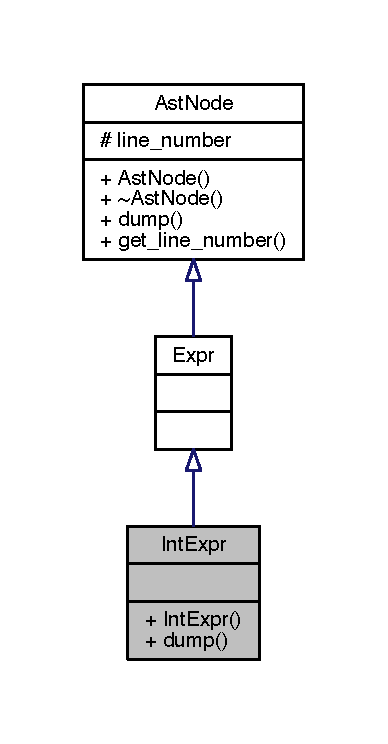
\includegraphics[width=186pt]{class_int_expr__inherit__graph}
\end{center}
\end{figure}


Collaboration diagram for Int\+Expr\+:\nopagebreak
\begin{figure}[H]
\begin{center}
\leavevmode
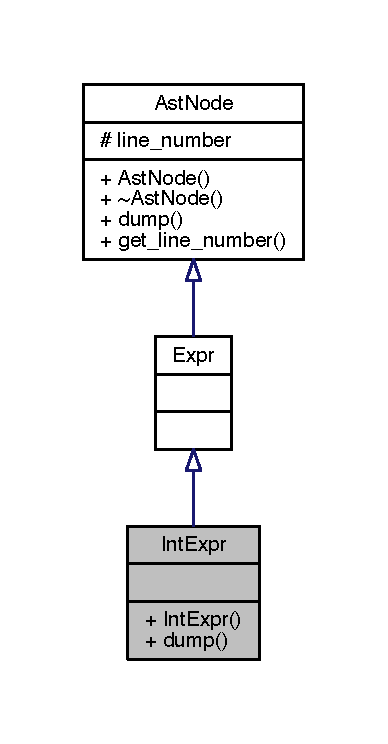
\includegraphics[width=186pt]{class_int_expr__coll__graph}
\end{center}
\end{figure}
\subsection*{Public Member Functions}
\begin{DoxyCompactItemize}
\item 
\mbox{\Hypertarget{class_int_expr_a0933883d5593409f38db273c27f21214}\label{class_int_expr_a0933883d5593409f38db273c27f21214}} 
{\bfseries Int\+Expr} (int n)
\item 
\mbox{\Hypertarget{class_int_expr_ad525807d1a1f843a548eda154135e136}\label{class_int_expr_ad525807d1a1f843a548eda154135e136}} 
virtual void {\bfseries dump} (ostream \&os, int n) override
\end{DoxyCompactItemize}
\subsection*{Additional Inherited Members}


The documentation for this class was generated from the following files\+:\begin{DoxyCompactItemize}
\item 
/\+Users/kevin/\+Code/sjtu/smallc/ast.\+h\item 
/\+Users/kevin/\+Code/sjtu/smallc/ast.\+cpp\end{DoxyCompactItemize}

\hypertarget{class_int_init}{}\section{Int\+Init Class Reference}
\label{class_int_init}\index{Int\+Init@{Int\+Init}}


Inheritance diagram for Int\+Init\+:\nopagebreak
\begin{figure}[H]
\begin{center}
\leavevmode
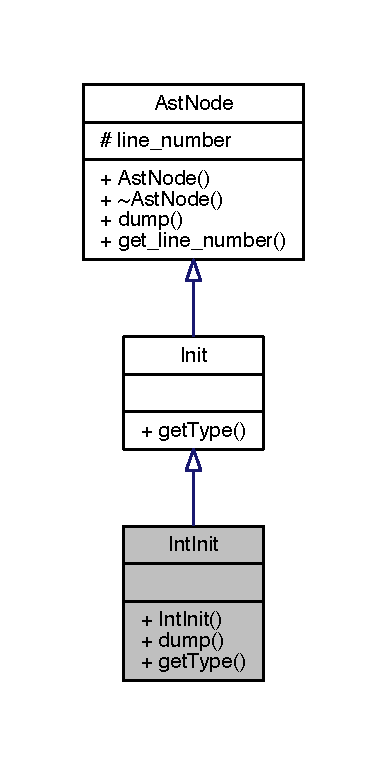
\includegraphics[width=186pt]{class_int_init__inherit__graph}
\end{center}
\end{figure}


Collaboration diagram for Int\+Init\+:\nopagebreak
\begin{figure}[H]
\begin{center}
\leavevmode
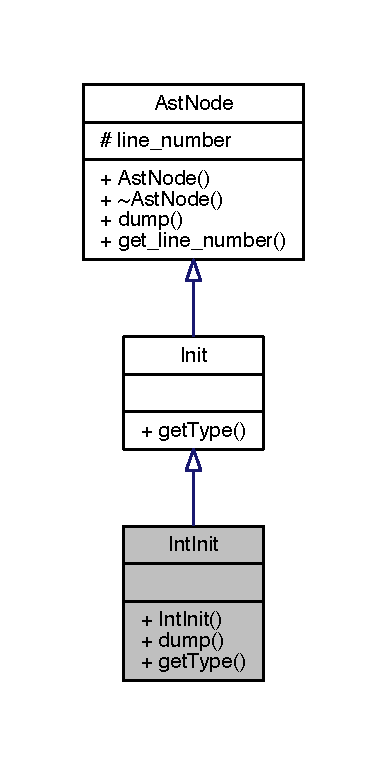
\includegraphics[width=186pt]{class_int_init__coll__graph}
\end{center}
\end{figure}
\subsection*{Public Member Functions}
\begin{DoxyCompactItemize}
\item 
\mbox{\Hypertarget{class_int_init_a901a68a61f2ddc6ea793ef14e7347a1e}\label{class_int_init_a901a68a61f2ddc6ea793ef14e7347a1e}} 
{\bfseries Int\+Init} (\hyperlink{class_expr}{Expr} $\ast$exp)
\item 
\mbox{\Hypertarget{class_int_init_a7c5c03fd5e739570544f72fd9f84bbbf}\label{class_int_init_a7c5c03fd5e739570544f72fd9f84bbbf}} 
virtual void {\bfseries dump} (ostream \&os, int n) override
\item 
\mbox{\Hypertarget{class_int_init_a94e524ddfcd5d7df7ed9b200484eaaef}\label{class_int_init_a94e524ddfcd5d7df7ed9b200484eaaef}} 
Expr\+Type\+::type {\bfseries get\+Type} () const override
\end{DoxyCompactItemize}
\subsection*{Additional Inherited Members}


The documentation for this class was generated from the following files\+:\begin{DoxyCompactItemize}
\item 
/\+Users/kevin/\+Code/sjtu/smallc/ast.\+h\item 
/\+Users/kevin/\+Code/sjtu/smallc/ast.\+cpp\end{DoxyCompactItemize}

\hypertarget{class_no_expr}{}\section{No\+Expr Class Reference}
\label{class_no_expr}\index{No\+Expr@{No\+Expr}}


Inheritance diagram for No\+Expr\+:\nopagebreak
\begin{figure}[H]
\begin{center}
\leavevmode
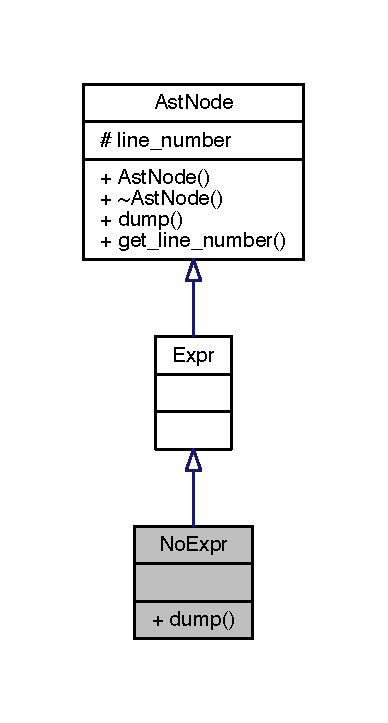
\includegraphics[width=186pt]{class_no_expr__inherit__graph}
\end{center}
\end{figure}


Collaboration diagram for No\+Expr\+:\nopagebreak
\begin{figure}[H]
\begin{center}
\leavevmode
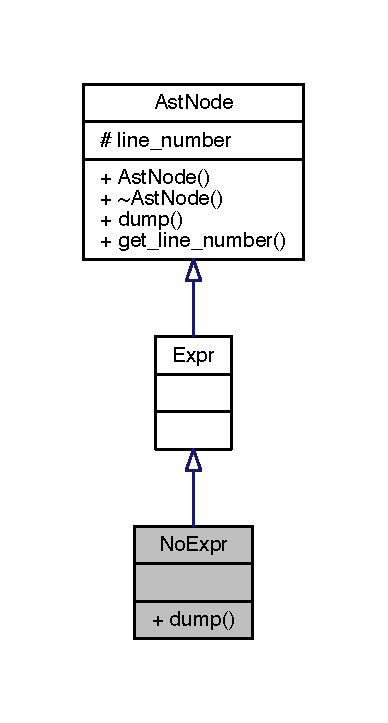
\includegraphics[width=186pt]{class_no_expr__coll__graph}
\end{center}
\end{figure}
\subsection*{Public Member Functions}
\begin{DoxyCompactItemize}
\item 
\mbox{\Hypertarget{class_no_expr_a9d91be9cce028a53f401efd69694826e}\label{class_no_expr_a9d91be9cce028a53f401efd69694826e}} 
virtual void {\bfseries dump} (ostream \&os, int n) override
\end{DoxyCompactItemize}
\subsection*{Additional Inherited Members}


The documentation for this class was generated from the following files\+:\begin{DoxyCompactItemize}
\item 
/\+Users/kevin/\+Code/sjtu/smallc/ast.\+h\item 
/\+Users/kevin/\+Code/sjtu/smallc/ast.\+cpp\end{DoxyCompactItemize}

\hypertarget{class_program}{}\section{Program Class Reference}
\label{class_program}\index{Program@{Program}}


{\ttfamily \#include $<$ast.\+h$>$}



Inheritance diagram for Program\+:\nopagebreak
\begin{figure}[H]
\begin{center}
\leavevmode
\includegraphics[width=186pt]{class_program__inherit__graph}
\end{center}
\end{figure}


Collaboration diagram for Program\+:\nopagebreak
\begin{figure}[H]
\begin{center}
\leavevmode
\includegraphics[width=186pt]{class_program__coll__graph}
\end{center}
\end{figure}
\subsection*{Public Member Functions}
\begin{DoxyCompactItemize}
\item 
\mbox{\Hypertarget{class_program_ab74fa81e40ae89ea91c6f14672526968}\label{class_program_ab74fa81e40ae89ea91c6f14672526968}} 
{\bfseries Program} (Ext\+Def\+List $\ast$defs)
\item 
void \hyperlink{class_program_a1fec659a1de541b94b87e17cad84f5a2}{semant} (ostream \&out)
\item 
\mbox{\Hypertarget{class_program_ab9a7906af6b6c07139fbf8c7cb44bdd1}\label{class_program_ab9a7906af6b6c07139fbf8c7cb44bdd1}} 
virtual void {\bfseries dump} (ostream \&os, int n) override
\end{DoxyCompactItemize}
\subsection*{Protected Attributes}
\begin{DoxyCompactItemize}
\item 
\mbox{\Hypertarget{class_program_a41ddedf2d23da68ca6f74163334adc2c}\label{class_program_a41ddedf2d23da68ca6f74163334adc2c}} 
Ext\+Def\+List $\ast$ {\bfseries extdefs}
\end{DoxyCompactItemize}


\subsection{Detailed Description}
P\+R\+O\+G\+R\+AM -\/$>$ E\+X\+T\+D\+E\+FS 

\subsection{Member Function Documentation}
\mbox{\Hypertarget{class_program_a1fec659a1de541b94b87e17cad84f5a2}\label{class_program_a1fec659a1de541b94b87e17cad84f5a2}} 
\index{Program@{Program}!semant@{semant}}
\index{semant@{semant}!Program@{Program}}
\subsubsection{\texorpdfstring{semant()}{semant()}}
{\footnotesize\ttfamily void Program\+::semant (\begin{DoxyParamCaption}\item[{ostream \&}]{out }\end{DoxyParamCaption})}



 \subsubsection*{Implementation of semant analysis }

The documentation for this class was generated from the following files\+:\begin{DoxyCompactItemize}
\item 
/\+Users/kevin/\+Code/sjtu/smallc/ast.\+h\item 
/\+Users/kevin/\+Code/sjtu/smallc/ast.\+cpp\item 
/\+Users/kevin/\+Code/sjtu/smallc/semant.\+cpp\end{DoxyCompactItemize}

\hypertarget{class_return_stmt}{}\section{Return\+Stmt Class Reference}
\label{class_return_stmt}\index{Return\+Stmt@{Return\+Stmt}}


Inheritance diagram for Return\+Stmt\+:\nopagebreak
\begin{figure}[H]
\begin{center}
\leavevmode
\includegraphics[width=186pt]{class_return_stmt__inherit__graph}
\end{center}
\end{figure}


Collaboration diagram for Return\+Stmt\+:\nopagebreak
\begin{figure}[H]
\begin{center}
\leavevmode
\includegraphics[width=186pt]{class_return_stmt__coll__graph}
\end{center}
\end{figure}
\subsection*{Public Member Functions}
\begin{DoxyCompactItemize}
\item 
\mbox{\Hypertarget{class_return_stmt_a1a7ddb42fa5a21f8718560e6feab3b2d}\label{class_return_stmt_a1a7ddb42fa5a21f8718560e6feab3b2d}} 
{\bfseries Return\+Stmt} (\hyperlink{class_expr}{Expr} $\ast$exp)
\item 
\mbox{\Hypertarget{class_return_stmt_a7182695c15dddd6f2f3dcefc6eb7c994}\label{class_return_stmt_a7182695c15dddd6f2f3dcefc6eb7c994}} 
virtual void {\bfseries dump} (ostream \&os, int n) override
\end{DoxyCompactItemize}
\subsection*{Additional Inherited Members}


The documentation for this class was generated from the following files\+:\begin{DoxyCompactItemize}
\item 
/\+Users/kevin/\+Code/sjtu/smallc/ast.\+h\item 
/\+Users/kevin/\+Code/sjtu/smallc/ast.\+cpp\end{DoxyCompactItemize}

\hypertarget{class_s_def}{}\section{S\+Def Class Reference}
\label{class_s_def}\index{S\+Def@{S\+Def}}


Inheritance diagram for S\+Def\+:\nopagebreak
\begin{figure}[H]
\begin{center}
\leavevmode
\includegraphics[width=186pt]{class_s_def__inherit__graph}
\end{center}
\end{figure}


Collaboration diagram for S\+Def\+:\nopagebreak
\begin{figure}[H]
\begin{center}
\leavevmode
\includegraphics[width=186pt]{class_s_def__coll__graph}
\end{center}
\end{figure}
\subsection*{Public Member Functions}
\begin{DoxyCompactItemize}
\item 
\mbox{\Hypertarget{class_s_def_a8497380a982313cef1b7c5bc59a28040}\label{class_s_def_a8497380a982313cef1b7c5bc59a28040}} 
{\bfseries S\+Def} (\hyperlink{class_struct_spec}{Struct\+Spec} $\ast$sts, S\+Dec\+List $\ast$sdl)
\item 
\mbox{\Hypertarget{class_s_def_afc37aa5d57ea94c75c3a08c01cbbc0d7}\label{class_s_def_afc37aa5d57ea94c75c3a08c01cbbc0d7}} 
virtual void {\bfseries dump} (ostream \&os, int n) override
\end{DoxyCompactItemize}
\subsection*{Additional Inherited Members}


The documentation for this class was generated from the following files\+:\begin{DoxyCompactItemize}
\item 
/\+Users/kevin/\+Code/sjtu/smallc/ast.\+h\item 
/\+Users/kevin/\+Code/sjtu/smallc/ast.\+cpp\end{DoxyCompactItemize}

\hypertarget{class_stmt}{}\section{Stmt Class Reference}
\label{class_stmt}\index{Stmt@{Stmt}}


{\ttfamily \#include $<$ast.\+h$>$}



Inheritance diagram for Stmt\+:\nopagebreak
\begin{figure}[H]
\begin{center}
\leavevmode
\includegraphics[width=350pt]{class_stmt__inherit__graph}
\end{center}
\end{figure}


Collaboration diagram for Stmt\+:\nopagebreak
\begin{figure}[H]
\begin{center}
\leavevmode
\includegraphics[width=186pt]{class_stmt__coll__graph}
\end{center}
\end{figure}
\subsection*{Additional Inherited Members}


\subsection{Detailed Description}
Statements

S\+T\+MT -\/$>$ E\+XP S\+E\+MI $\sim$ \hyperlink{class_expr_stmt}{Expr\+Stmt} $\vert$ S\+T\+M\+T\+B\+L\+O\+CK $\sim$ \hyperlink{class_stmt_block}{Stmt\+Block} $\vert$ R\+E\+T\+U\+RN E\+XP S\+E\+MI $\sim$ \hyperlink{class_return_stmt}{Return\+Stmt} $\vert$ IF LP E\+XP RP S\+T\+MT $\sim$ \hyperlink{class_if_stmt}{If\+Stmt} $\vert$ IF LP E\+XP RP S\+T\+MT E\+L\+SE S\+T\+MT $\sim$ \hyperlink{class_if_stmt}{If\+Stmt} $\vert$ F\+OR LP E\+XP S\+E\+MI E\+XP S\+E\+MI E\+XP RP S\+T\+MT $\sim$ \hyperlink{class_for_stmt}{For\+Stmt} $\vert$ C\+O\+NT S\+E\+MI $\sim$ \hyperlink{class_cont_stmt}{Cont\+Stmt} $\vert$ B\+R\+E\+AK S\+E\+MI $\sim$ \hyperlink{class_break_stmt}{Break\+Stmt} 

The documentation for this class was generated from the following file\+:\begin{DoxyCompactItemize}
\item 
/\+Users/kevin/\+Code/sjtu/smallc/ast.\+h\end{DoxyCompactItemize}

\hypertarget{class_stmt_block}{}\section{Stmt\+Block Class Reference}
\label{class_stmt_block}\index{Stmt\+Block@{Stmt\+Block}}


{\ttfamily \#include $<$ast.\+h$>$}



Inheritance diagram for Stmt\+Block\+:\nopagebreak
\begin{figure}[H]
\begin{center}
\leavevmode
\includegraphics[width=186pt]{class_stmt_block__inherit__graph}
\end{center}
\end{figure}


Collaboration diagram for Stmt\+Block\+:\nopagebreak
\begin{figure}[H]
\begin{center}
\leavevmode
\includegraphics[width=186pt]{class_stmt_block__coll__graph}
\end{center}
\end{figure}
\subsection*{Public Member Functions}
\begin{DoxyCompactItemize}
\item 
\mbox{\Hypertarget{class_stmt_block_ae2de3b72f160c22ea471670ed543d94b}\label{class_stmt_block_ae2de3b72f160c22ea471670ed543d94b}} 
{\bfseries Stmt\+Block} (Def\+List $\ast$dl, Stmt\+List $\ast$sl)
\item 
\mbox{\Hypertarget{class_stmt_block_a0fa1df31741ba3e835bbc052f9814d62}\label{class_stmt_block_a0fa1df31741ba3e835bbc052f9814d62}} 
virtual void {\bfseries dump} (ostream \&os, int n) override
\end{DoxyCompactItemize}
\subsection*{Additional Inherited Members}


\subsection{Detailed Description}
Statement block

S\+T\+M\+T\+B\+L\+O\+CK -\/$>$ LC D\+E\+FS S\+T\+M\+TS RC 

The documentation for this class was generated from the following files\+:\begin{DoxyCompactItemize}
\item 
/\+Users/kevin/\+Code/sjtu/smallc/ast.\+h\item 
/\+Users/kevin/\+Code/sjtu/smallc/ast.\+cpp\end{DoxyCompactItemize}

\hypertarget{class_struct_def}{}\section{Struct\+Def Class Reference}
\label{class_struct_def}\index{Struct\+Def@{Struct\+Def}}


{\ttfamily \#include $<$ast.\+h$>$}



Inheritance diagram for Struct\+Def\+:\nopagebreak
\begin{figure}[H]
\begin{center}
\leavevmode
\includegraphics[width=186pt]{class_struct_def__inherit__graph}
\end{center}
\end{figure}


Collaboration diagram for Struct\+Def\+:\nopagebreak
\begin{figure}[H]
\begin{center}
\leavevmode
\includegraphics[width=186pt]{class_struct_def__coll__graph}
\end{center}
\end{figure}
\subsection*{Public Member Functions}
\begin{DoxyCompactItemize}
\item 
\mbox{\Hypertarget{class_struct_def_aa4e355dd27ce1343f4f38e8032b2cd43}\label{class_struct_def_aa4e355dd27ce1343f4f38e8032b2cd43}} 
{\bfseries Struct\+Def} (S\+Dec\+List $\ast$sdl)
\item 
\mbox{\Hypertarget{class_struct_def_a107958af5eb5e2b4034960fd6b90ad99}\label{class_struct_def_a107958af5eb5e2b4034960fd6b90ad99}} 
virtual void {\bfseries dump} (ostream \&os, int n) override
\end{DoxyCompactItemize}
\subsection*{Additional Inherited Members}


\subsection{Detailed Description}
S\+D\+EF -\/$>$ T\+Y\+PE S\+D\+E\+CS S\+E\+MI

only I\+NT is supported as T\+Y\+PE. 

The documentation for this class was generated from the following files\+:\begin{DoxyCompactItemize}
\item 
/\+Users/kevin/\+Code/sjtu/smallc/ast.\+h\item 
/\+Users/kevin/\+Code/sjtu/smallc/ast.\+cpp\end{DoxyCompactItemize}

\hypertarget{class_struct_ext_def}{}\section{Struct\+Ext\+Def Class Reference}
\label{class_struct_ext_def}\index{Struct\+Ext\+Def@{Struct\+Ext\+Def}}


{\ttfamily \#include $<$ast.\+h$>$}



Inheritance diagram for Struct\+Ext\+Def\+:\nopagebreak
\begin{figure}[H]
\begin{center}
\leavevmode
\includegraphics[width=186pt]{class_struct_ext_def__inherit__graph}
\end{center}
\end{figure}


Collaboration diagram for Struct\+Ext\+Def\+:\nopagebreak
\begin{figure}[H]
\begin{center}
\leavevmode
\includegraphics[width=186pt]{class_struct_ext_def__coll__graph}
\end{center}
\end{figure}
\subsection*{Public Member Functions}
\begin{DoxyCompactItemize}
\item 
\mbox{\Hypertarget{class_struct_ext_def_aa5d2a48a60a50596627ad52bdf5099b5}\label{class_struct_ext_def_aa5d2a48a60a50596627ad52bdf5099b5}} 
{\bfseries Struct\+Ext\+Def} (\hyperlink{class_struct_spec}{Struct\+Spec} $\ast$st, S\+Ext\+Var\+List $\ast$slist)
\item 
\mbox{\Hypertarget{class_struct_ext_def_abae4ce32fa80590d46598e210ffd2350}\label{class_struct_ext_def_abae4ce32fa80590d46598e210ffd2350}} 
virtual void {\bfseries dump} (ostream \&os, int n) override
\item 
\mbox{\Hypertarget{class_struct_ext_def_ac518c458ea78fa240de2ee9db61c22f9}\label{class_struct_ext_def_ac518c458ea78fa240de2ee9db61c22f9}} 
void {\bfseries check} () override
\end{DoxyCompactItemize}
\subsection*{Additional Inherited Members}


\subsection{Detailed Description}
Struct defs

E\+X\+T\+D\+EF -\/$>$ S\+T\+S\+P\+EC S\+E\+X\+T\+V\+A\+RS S\+E\+MI 

The documentation for this class was generated from the following files\+:\begin{DoxyCompactItemize}
\item 
/\+Users/kevin/\+Code/sjtu/smallc/ast.\+h\item 
/\+Users/kevin/\+Code/sjtu/smallc/ast.\+cpp\end{DoxyCompactItemize}

\hypertarget{class_struct_spec}{}\section{Struct\+Spec Class Reference}
\label{class_struct_spec}\index{Struct\+Spec@{Struct\+Spec}}


{\ttfamily \#include $<$ast.\+h$>$}



Inheritance diagram for Struct\+Spec\+:\nopagebreak
\begin{figure}[H]
\begin{center}
\leavevmode
\includegraphics[width=186pt]{class_struct_spec__inherit__graph}
\end{center}
\end{figure}


Collaboration diagram for Struct\+Spec\+:\nopagebreak
\begin{figure}[H]
\begin{center}
\leavevmode
\includegraphics[width=186pt]{class_struct_spec__coll__graph}
\end{center}
\end{figure}
\subsection*{Public Member Functions}
\begin{DoxyCompactItemize}
\item 
\mbox{\Hypertarget{class_struct_spec_a40337f31924605b272f59cf74c8369f7}\label{class_struct_spec_a40337f31924605b272f59cf74c8369f7}} 
{\bfseries Struct\+Spec} (string id)
\item 
\mbox{\Hypertarget{class_struct_spec_aadfa6e7e14621e2bce084171ac8808a1}\label{class_struct_spec_aadfa6e7e14621e2bce084171ac8808a1}} 
{\bfseries Struct\+Spec} (string id, St\+Def\+List $\ast$sl)
\item 
\mbox{\Hypertarget{class_struct_spec_af0ed4377c426336943b18090876a20eb}\label{class_struct_spec_af0ed4377c426336943b18090876a20eb}} 
{\bfseries Struct\+Spec} (St\+Def\+List $\ast$sl)
\item 
\mbox{\Hypertarget{class_struct_spec_a3bff556be3067bf2258730883e72c1a3}\label{class_struct_spec_a3bff556be3067bf2258730883e72c1a3}} 
virtual void {\bfseries dump} (ostream \&os, int n) override
\end{DoxyCompactItemize}
\subsection*{Additional Inherited Members}


\subsection{Detailed Description}
\hyperlink{class_struct_spec}{Struct\+Spec}

S\+T\+S\+P\+EC -\/$>$ S\+T\+R\+U\+CT ID LC S\+D\+E\+FS RC $\vert$ S\+T\+R\+U\+CT LC S\+D\+E\+FS RC $\vert$ S\+T\+R\+U\+CT ID; 

The documentation for this class was generated from the following files\+:\begin{DoxyCompactItemize}
\item 
/\+Users/kevin/\+Code/sjtu/smallc/ast.\+h\item 
/\+Users/kevin/\+Code/sjtu/smallc/ast.\+cpp\end{DoxyCompactItemize}

\hypertarget{class_symbol_table}{}\section{Symbol\+Table$<$ D\+AT $>$ Class Template Reference}
\label{class_symbol_table}\index{Symbol\+Table$<$ D\+A\+T $>$@{Symbol\+Table$<$ D\+A\+T $>$}}


Collaboration diagram for Symbol\+Table$<$ D\+AT $>$\+:\nopagebreak
\begin{figure}[H]
\begin{center}
\leavevmode
\includegraphics[width=190pt]{class_symbol_table__coll__graph}
\end{center}
\end{figure}
\subsection*{Public Member Functions}
\begin{DoxyCompactItemize}
\item 
\mbox{\Hypertarget{class_symbol_table_a13a91c38adca7a32c0c79573f7286f5b}\label{class_symbol_table_a13a91c38adca7a32c0c79573f7286f5b}} 
\hyperlink{class_symbol_table}{Symbol\+Table} \& {\bfseries operator=} (const \hyperlink{class_symbol_table}{Symbol\+Table} \&s)
\item 
\mbox{\Hypertarget{class_symbol_table_a08cecd4ea775f2ef78eeff19eadac32f}\label{class_symbol_table_a08cecd4ea775f2ef78eeff19eadac32f}} 
void {\bfseries fatal\+\_\+error} (string msg)
\item 
\mbox{\Hypertarget{class_symbol_table_a7a7f91a10ecd02760523919219f49492}\label{class_symbol_table_a7a7f91a10ecd02760523919219f49492}} 
void {\bfseries enterscope} ()
\item 
\mbox{\Hypertarget{class_symbol_table_aae704765597a4da4d763cf018afcd07a}\label{class_symbol_table_aae704765597a4da4d763cf018afcd07a}} 
void {\bfseries exitscope} ()
\item 
\mbox{\Hypertarget{class_symbol_table_a9b7b92cd9be9fff7a042ce5fe8eb12f3}\label{class_symbol_table_a9b7b92cd9be9fff7a042ce5fe8eb12f3}} 
void {\bfseries put} (string s, D\+AT i)
\item 
\mbox{\Hypertarget{class_symbol_table_a68e684fe62e86c8527e56e619dadd307}\label{class_symbol_table_a68e684fe62e86c8527e56e619dadd307}} 
D\+AT {\bfseries lookup} (string s)
\item 
\mbox{\Hypertarget{class_symbol_table_a046c3b1432ba64cfdaa429e035ca7f8c}\label{class_symbol_table_a046c3b1432ba64cfdaa429e035ca7f8c}} 
D\+AT {\bfseries probe} (string s)
\item 
\mbox{\Hypertarget{class_symbol_table_abe94f148c8fb2c2a4985b40ef3a0fd6a}\label{class_symbol_table_abe94f148c8fb2c2a4985b40ef3a0fd6a}} 
void {\bfseries dump} ()
\end{DoxyCompactItemize}


The documentation for this class was generated from the following file\+:\begin{DoxyCompactItemize}
\item 
/\+Users/kevin/\+Code/sjtu/smallc/symtab.\+h\end{DoxyCompactItemize}

\hypertarget{class_uop_expr}{}\section{Uop\+Expr Class Reference}
\label{class_uop_expr}\index{Uop\+Expr@{Uop\+Expr}}


Inheritance diagram for Uop\+Expr\+:\nopagebreak
\begin{figure}[H]
\begin{center}
\leavevmode
\includegraphics[width=186pt]{class_uop_expr__inherit__graph}
\end{center}
\end{figure}


Collaboration diagram for Uop\+Expr\+:\nopagebreak
\begin{figure}[H]
\begin{center}
\leavevmode
\includegraphics[width=186pt]{class_uop_expr__coll__graph}
\end{center}
\end{figure}
\subsection*{Public Member Functions}
\begin{DoxyCompactItemize}
\item 
\mbox{\Hypertarget{class_uop_expr_afee1fe4e395a5e78a00da75a392b6412}\label{class_uop_expr_afee1fe4e395a5e78a00da75a392b6412}} 
{\bfseries Uop\+Expr} (string op, \hyperlink{class_expr}{Expr} $\ast$exp)
\item 
\mbox{\Hypertarget{class_uop_expr_ab784d7b27f994ea2182d89bf430759a2}\label{class_uop_expr_ab784d7b27f994ea2182d89bf430759a2}} 
virtual void {\bfseries dump} (ostream \&os, int n) override
\end{DoxyCompactItemize}
\subsection*{Additional Inherited Members}


The documentation for this class was generated from the following files\+:\begin{DoxyCompactItemize}
\item 
/\+Users/kevin/\+Code/sjtu/smallc/ast.\+h\item 
/\+Users/kevin/\+Code/sjtu/smallc/ast.\+cpp\end{DoxyCompactItemize}

\hypertarget{class_var}{}\section{Var Class Reference}
\label{class_var}\index{Var@{Var}}


{\ttfamily \#include $<$ast.\+h$>$}



Inheritance diagram for Var\+:\nopagebreak
\begin{figure}[H]
\begin{center}
\leavevmode
\includegraphics[width=234pt]{class_var__inherit__graph}
\end{center}
\end{figure}


Collaboration diagram for Var\+:\nopagebreak
\begin{figure}[H]
\begin{center}
\leavevmode
\includegraphics[width=186pt]{class_var__coll__graph}
\end{center}
\end{figure}
\subsection*{Public Member Functions}
\begin{DoxyCompactItemize}
\item 
\mbox{\Hypertarget{class_var_ae7b58bfb649ef44ae9ac3cc33a6b39c4}\label{class_var_ae7b58bfb649ef44ae9ac3cc33a6b39c4}} 
virtual Expr\+Type\+::type {\bfseries get\+Type} () const =0
\end{DoxyCompactItemize}
\subsection*{Additional Inherited Members}


\subsection{Detailed Description}
\hyperlink{class_var}{Var}

V\+AR -\/$>$ ID $\sim$ \hyperlink{class_id_var}{Id\+Var} $\vert$ V\+AR LB I\+N\+IT RB $\sim$ \hyperlink{class_array_var}{Array\+Var} 

The documentation for this class was generated from the following file\+:\begin{DoxyCompactItemize}
\item 
/\+Users/kevin/\+Code/sjtu/smallc/ast.\+h\end{DoxyCompactItemize}

\hypertarget{class_var_def}{}\section{Var\+Def Class Reference}
\label{class_var_def}\index{Var\+Def@{Var\+Def}}


Inheritance diagram for Var\+Def\+:\nopagebreak
\begin{figure}[H]
\begin{center}
\leavevmode
\includegraphics[width=186pt]{class_var_def__inherit__graph}
\end{center}
\end{figure}


Collaboration diagram for Var\+Def\+:\nopagebreak
\begin{figure}[H]
\begin{center}
\leavevmode
\includegraphics[width=186pt]{class_var_def__coll__graph}
\end{center}
\end{figure}
\subsection*{Public Member Functions}
\begin{DoxyCompactItemize}
\item 
\mbox{\Hypertarget{class_var_def_a84d598952d4bba93b5798b62001b679d}\label{class_var_def_a84d598952d4bba93b5798b62001b679d}} 
{\bfseries Var\+Def} (Dec\+List $\ast$dl)
\item 
\mbox{\Hypertarget{class_var_def_aab9d4538a24c88690974f1ed3ea1ab08}\label{class_var_def_aab9d4538a24c88690974f1ed3ea1ab08}} 
virtual void {\bfseries dump} (ostream \&os, int n) override
\end{DoxyCompactItemize}
\subsection*{Additional Inherited Members}


The documentation for this class was generated from the following files\+:\begin{DoxyCompactItemize}
\item 
/\+Users/kevin/\+Code/sjtu/smallc/ast.\+h\item 
/\+Users/kevin/\+Code/sjtu/smallc/ast.\+cpp\end{DoxyCompactItemize}

\hypertarget{class_var_ext_def}{}\section{Var\+Ext\+Def Class Reference}
\label{class_var_ext_def}\index{Var\+Ext\+Def@{Var\+Ext\+Def}}


{\ttfamily \#include $<$ast.\+h$>$}



Inheritance diagram for Var\+Ext\+Def\+:\nopagebreak
\begin{figure}[H]
\begin{center}
\leavevmode
\includegraphics[width=186pt]{class_var_ext_def__inherit__graph}
\end{center}
\end{figure}


Collaboration diagram for Var\+Ext\+Def\+:\nopagebreak
\begin{figure}[H]
\begin{center}
\leavevmode
\includegraphics[width=186pt]{class_var_ext_def__coll__graph}
\end{center}
\end{figure}
\subsection*{Public Member Functions}
\begin{DoxyCompactItemize}
\item 
\mbox{\Hypertarget{class_var_ext_def_a8ba52350a3f35cb8eeafbdb678df5ea9}\label{class_var_ext_def_a8ba52350a3f35cb8eeafbdb678df5ea9}} 
{\bfseries Var\+Ext\+Def} (Ext\+Var\+List $\ast$extvars)
\item 
\mbox{\Hypertarget{class_var_ext_def_af91ffac816eca11ee3dde6c454cad868}\label{class_var_ext_def_af91ffac816eca11ee3dde6c454cad868}} 
virtual void {\bfseries dump} (ostream \&os, int n) override
\item 
\mbox{\Hypertarget{class_var_ext_def_aaa89f410f59265cf9f5d2317ae261aa8}\label{class_var_ext_def_aaa89f410f59265cf9f5d2317ae261aa8}} 
void {\bfseries check} () override
\end{DoxyCompactItemize}
\subsection*{Additional Inherited Members}


\subsection{Detailed Description}
Variable defs;

E\+X\+T\+D\+EF -\/$>$ T\+Y\+PE E\+X\+T\+V\+A\+RS S\+E\+MI 

The documentation for this class was generated from the following files\+:\begin{DoxyCompactItemize}
\item 
/\+Users/kevin/\+Code/sjtu/smallc/ast.\+h\item 
/\+Users/kevin/\+Code/sjtu/smallc/ast.\+cpp\item 
/\+Users/kevin/\+Code/sjtu/smallc/semant.\+cpp\end{DoxyCompactItemize}

%--- End generated contents ---

% Index
\backmatter
\newpage
\phantomsection
\clearemptydoublepage
\addcontentsline{toc}{chapter}{Index}
\printindex

\end{document}
